%%%%%%%%%%%%%%%%%%%%%%%%%%%%%%%%%%%%%%%%%%%%%%%%%%
%  JASA LaTeX Template File
%  To make articles using JASA.cls, Version 1.1
%  September 14, 2019
%%%%%%%%%%%%%%%%%%%%%%%%%%%%%%%%%%%%%%%%%%%%%%%%%%

%% Step 1:
%% Uncomment the style that you want to use:

%%%%%%% For Preprint
%% For manuscript, 12pt, one column style

\documentclass[reprint]{JASA}

%%%%% Preprint Options %%%%%
%% The track changes option allows you to mark changes
%% and will produce a list of changes, their line number
%% and page number at the end of the article.
%\documentclass[preprint,trackchanges]{JASA}


%% NumberedRefs is used for numbered bibliography and citations.
%% Default is Author-Year style.
%% \documentclass[preprint,NumberedRefs]{JASA}

%%%%%%% For Reprint
%% For appearance of finished article; 2 columns, 10 pt fonts

% \documentclass[reprint]{JASA}

%%%%% Reprint Options %%%%%

%% For testing to see if author has exceeded page length request, use 12pt option
%\documentclass[reprint,12pt]{JASA}


%% NumberedRefs is used for numbered bibliography and citations.
%% Default is Author-Year style.
% \documentclass[reprint,NumberedRefs]{JASA}

%% TurnOnLineNumbers
%% Make lines be numbered in reprint style:
% \documentclass[reprint,TurnOnLineNumbers]{JASA}

\usepackage{natbib}



% tightlist command for lists without linebreak
\providecommand{\tightlist}{%
  \setlength{\itemsep}{0pt}\setlength{\parskip}{0pt}}





\begin{document}
%% the square bracket argument will send term to running head in
%% preprint, or running foot in reprint style.

\title[]{Model-Based Similarity Scores for the Comparison of Cartridge
Case Impressions}

% ie
%\title[JASA/Sample JASA Article]{Sample JASA Article}

%% repeat as needed

\author{Joseph Zemmels}
% ie
%\affiliation{Department1,  University1, City, State ZipCode, Country}
\affiliation{Iowa State University}
%% for corresponding author
\email{jzemmels@iastate.edu}
%% for additional information
\thanks{other info}
\author{Heike Hofmann}
% ie
%\affiliation{Department1,  University1, City, State ZipCode, Country}
\affiliation{Iowa State University}
%% for corresponding author

%% for additional information

\author{Susan VanderPlas}
% ie
%\affiliation{Department1,  University1, City, State ZipCode, Country}
\affiliation{University of Nebraska - Lincoln}
%% for corresponding author

%% for additional information


% ie
% \author{Author Four}
% \email{author.four@university.edu}
% \thanks{Also at Another University, City, State ZipCode, Country.}

%% For preprint only,
%  optional, if you want want this message to appear in upper left corner of title page
\preprint{Zemmels, Hofmann, and VanderPlas, Statistical Analysis and
Data Mining}

%ie
%\preprint{Author, JASA}

% optional, if desired:
%\date{\today}
\date{\today}

\begin{abstract}
% Put your abstract here. Abstracts are limited to 200 words for
% regular articles and 100 words for Letters to the Editor. Please no
% personal pronouns, also please do not use the words ``new'' and/or
% ``novel'' in the abstract. An article usually includes an abstract, a
% concise summary of the work covered at length in the main body of the
% article.
Put your abstract here.
\end{abstract}

%% pacs numbers not used

\maketitle

%  End of title page for Preprint option --------------------------------- %

%% See preprint.tex/.pdf or reprint.tex/.pdf for many examples


%  Body of the article
\defcitealias{council_strengthening_2009}{NRC (2009)}
\defcitealias{pcast2016}{PCAST (2016)}

\hypertarget{introduction}{%
\section{Background \& Introduction}\label{introduction}}

A \emph{cartride case} is the part of firearm ammunition that houses the
projectile and propulsive device. When a firearm is discharged and the
projectile travels down the barrel, the cartridge case moves in the
opposite direction and slams against the back wall, the \emph{breech
face}, of the firearm. Markings on the breech face are ``stamped'' into
the surface of the cartridge case leaving so-called \emph{breech face
impressions}. In this paper, we introduce an automatic method for
measuring the similarity between two cartridge cases based on their
breech face impressions.

\hypertarget{traditional-cartridge-case-comparison}{%
\subsection{Traditional Cartridge Case
Comparison}\label{traditional-cartridge-case-comparison}}

In a traditional examination, forensic examiners use these impressions
analogous to a fingerprint to determine whether two cartridge cases were
fired from the same firearm. First, two cartridge cases are collected -
perhaps one is from a crime scene and the other is collected from a
suspect's gun. An examiner places the two cartridge cases beneath a
``comparison microscope'' that merges the views of two compound
microscopes into a single split view \citep{Thompson2017}. The examiner
assesses the ``degree of similarity'' between the markings on the
cartridge cases and reaches either an \emph{identification}, meaning the
cartridge cases were fired from the same firearm, an \emph{elimination},
meaning they were fired from different firearms, or an
\emph{inconclusive}, meaning the evidence is insufficient to make an
identification or elimination \citep{AFTE1992}.\footnote{The AFTE range
  of conclusions also permits the examiner to decide that the evidence
  is \emph{unsuitable} for examination, which can occur if evidence
  quality is poor; for example, a fragment of a cartridge case is
  recovered rather than a full cartridge case.}

Critics of traditional forensic examinations cite a lack of
``foundational validity'' underlying the procedures used by firearm and
toolmark examiners \citep{council_strengthening_2009, pcast2016}. In
particular, examiners rely largely on their subjective findings rather
than on a well-defined procedure to measure similarity.
\citetalias{pcast2016} pushed for ``developing and testing
image-analysis algorithms'' to objectively measure the similarity
between cartridge cases.

In this paper, we introduce a procedure to automatically compare digital
scans of cartridge cases. Throughout this paper, we use scans, taken by
us \textbf{{[}scientific data citation{]}}, of cartridge cases collected
by \citet{Baldwin2014}. The cartridge case scans are available as part
of the data repository at
\url{https://www.doi.org/10.25380/IASTATE.23837100.V1}
\citep{cartridgeCaseData}. We also provide code to reproduce the results
shared in this paper at
\url{https://github.com/jzemmels/rules_vs_scores}.

\hypertarget{algorithmic-cartridge-case-comparisons}{%
\subsection{Algorithmic Cartridge Case
Comparisons}\label{algorithmic-cartridge-case-comparisons}}

\hypertarget{cartridge-case-surface-scans}{%
\subsubsection{Cartridge Case Surface
Scans}\label{cartridge-case-surface-scans}}

We captured digital representations of cartridge case surfaces using
topographic scanning technology. The scanner measures the relative
surface depth and stores these measurements in a 2D array called a
\emph{surface matrix}. The left side of \autoref{fig:preProcessEffect}
depicts a surface matrix representing the region at the base of a
cartridge case surface called the \emph{primer}, which is the circular
metal cap struck by the firing pin to initiate the firing process. The
purple ring near the edges of the scan represent the boundary of the
cartridge case primer while the darker orange ring near the center of
the scan represents the deformation of metal caused by the contact with
the firing pin.

Of particular interest is the annular breech face impression region
around the firing pin impression. We isolate this region by applying a
series of manual and automatic pre-processing steps to the surface
matrix, resulting in the scan on the right side of
\autoref{fig:preProcessEffect}. The gray pixels in this image represent
structurally missing values introduced during pre-processing. See
\textbf{{[}scientific data citation{]}} for more information on the
pre-processing procedure.

\begin{figure}[htbp]
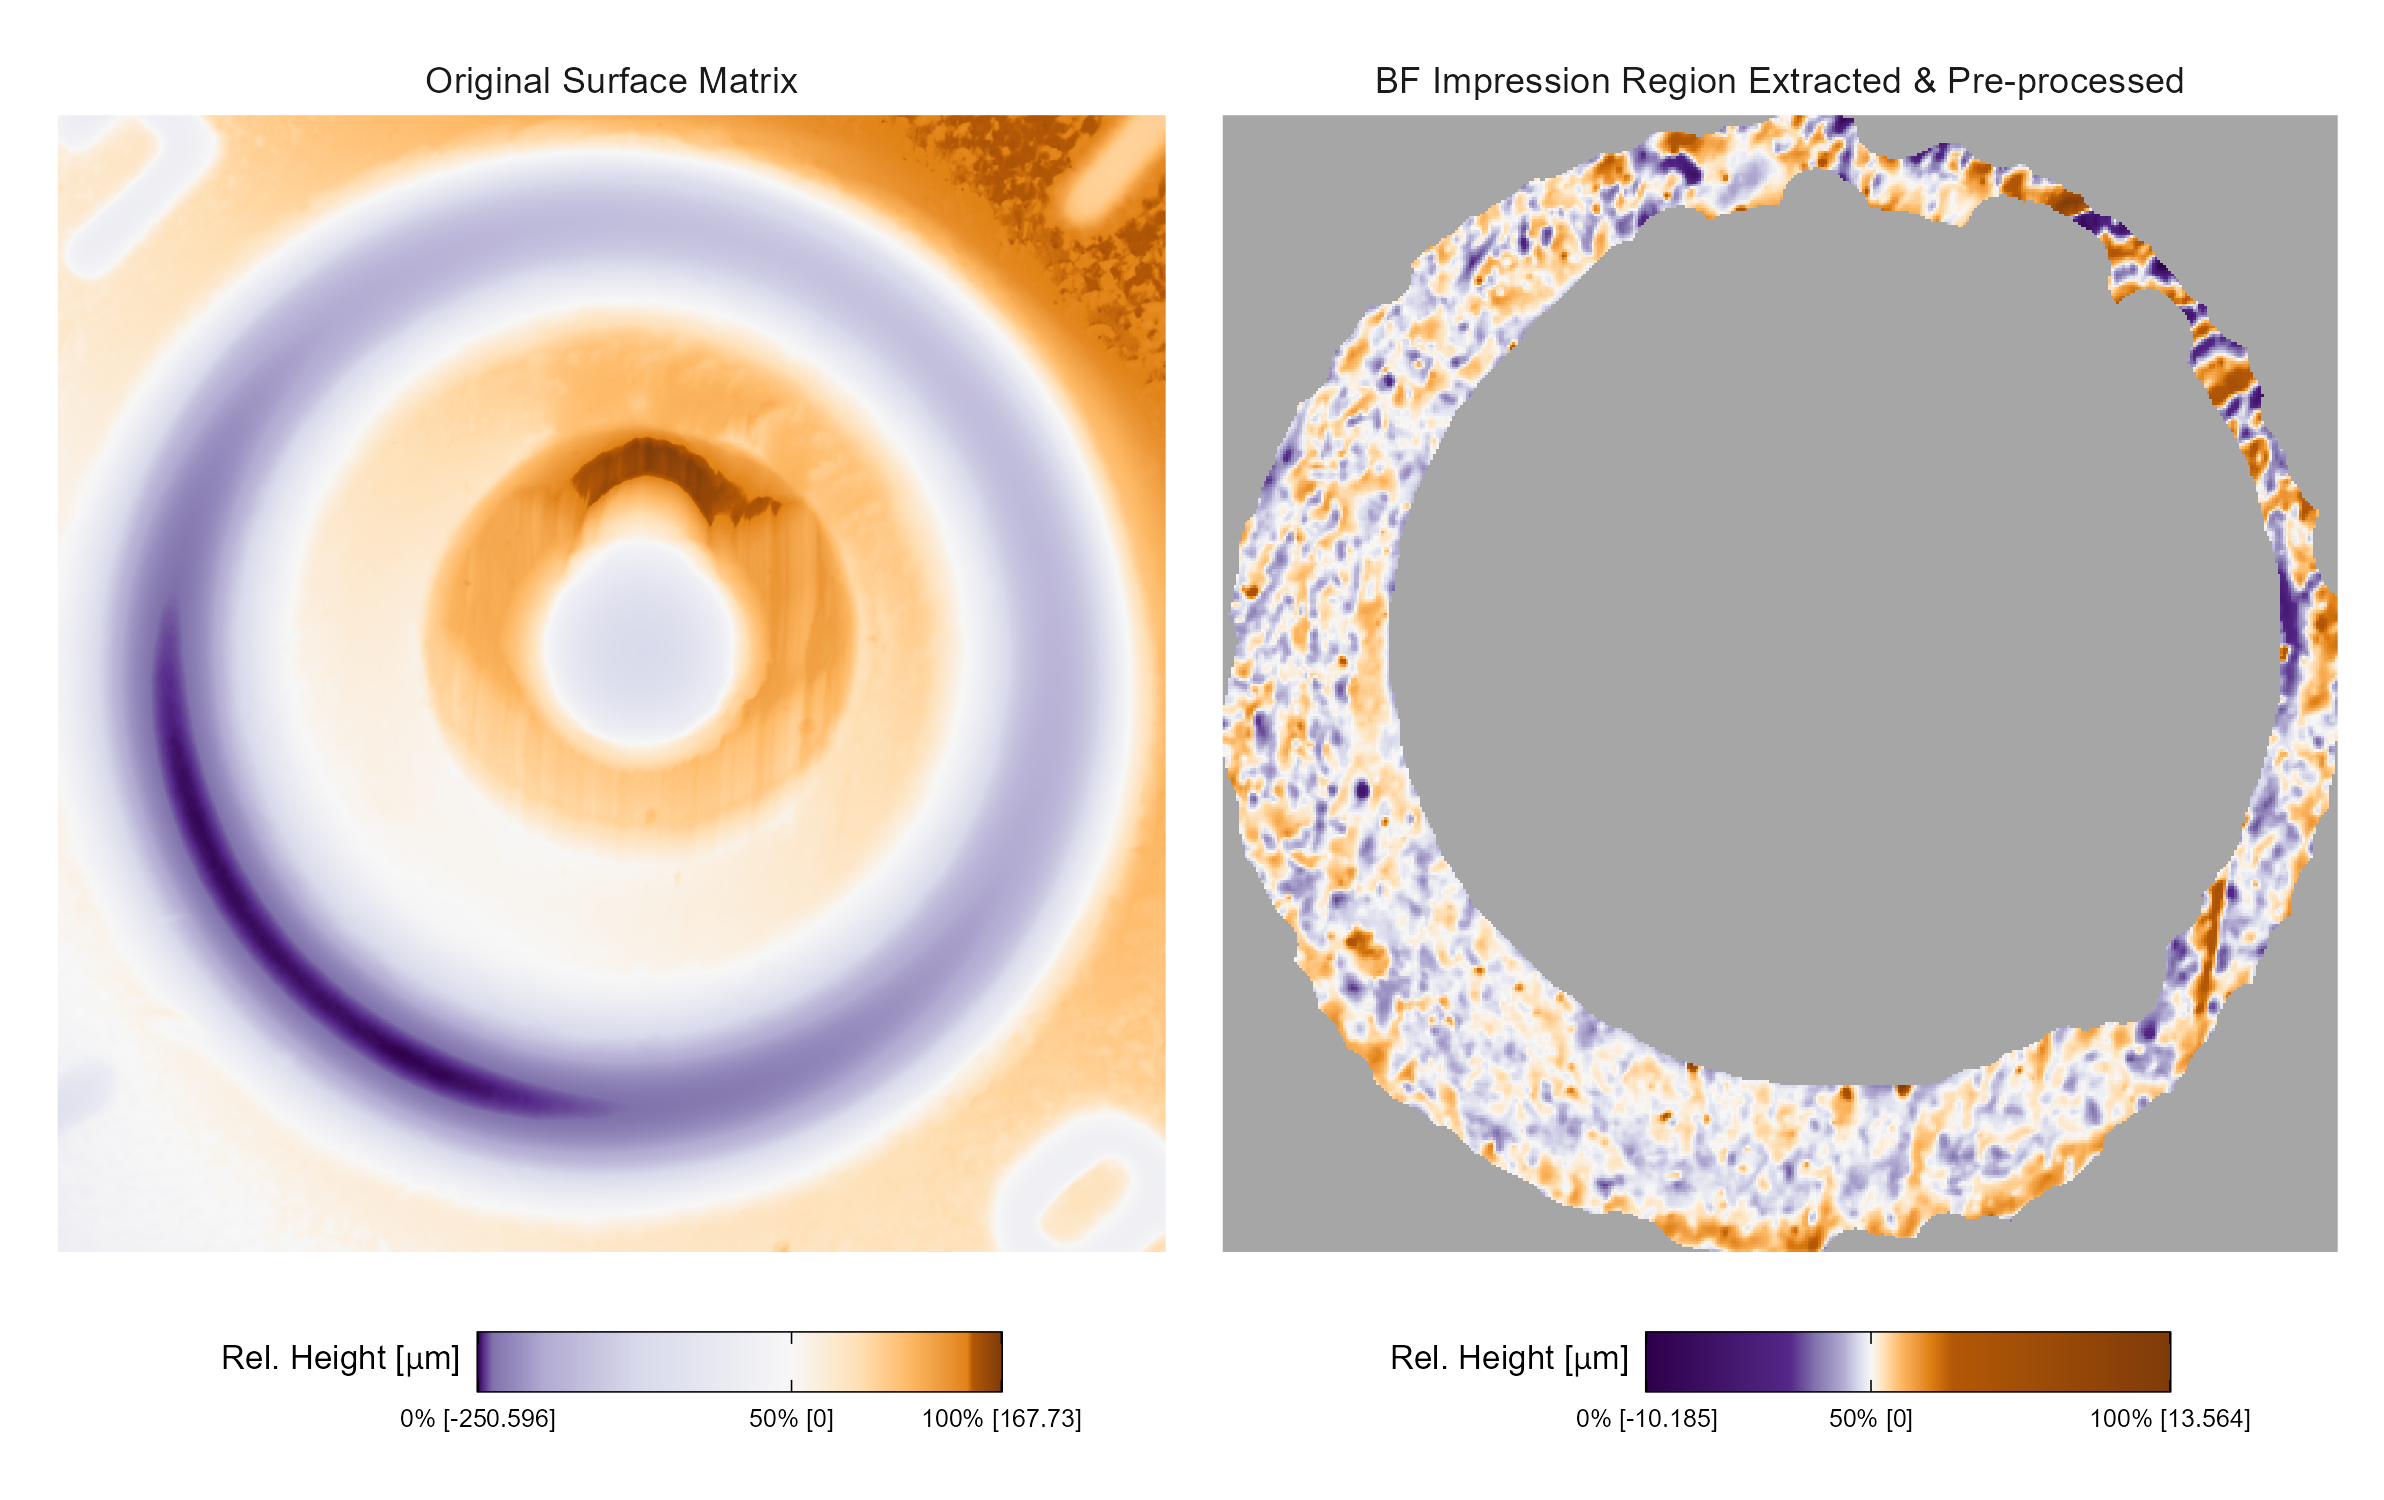
\includegraphics[width=.5\textwidth]{figures/preProcessEffect} \caption{\label{fig:preProcessEffect} We apply a sequence of pre-processing functions to each scan. Each pre-processing step further emphasizes the breech face impressions in the scan.}\label{fig:unnamed-chunk-1}
\end{figure}

Two pre-processed cartridge cases are compared to measure the similarity
of their breech face impressions. In the next section, we summarize a
technique for comparing cartridge case scans called the \emph{Congruent
Matching Cells} algorithm \citep{song_proposed_2013}.

\hypertarget{congruent-matching-cells-algorithm}{%
\subsubsection{Congruent Matching Cells
Algorithm}\label{congruent-matching-cells-algorithm}}

Recent proposals for automatic cartridge case scoring algorithms borrow
from image processing and computer vision techniques. For example,
\citet{vorburger_surface_2007} proposed using the cross-correlation
function (CCF) to compare images or scans of cartridge case surfaces.
The CCF measures the similarity between two matrices for all possible
translations of one matrix against the other. Calculating the CCF while
rotating one of the scans therefore allows for estimation of the optimal
translation and rotation, together referred to as the
\emph{registration}, between the two scans; simply choose the
rotation/translation at which the CCF is maximized.

\citet{song_proposed_2013} noted that two matching cartridge cases often
share similar impressions in specific regions, so calculating the CCF
between two full scans may not highlight their similarities. Instead,
\citet{song_proposed_2013} proposed partitioning one cartridge case scan
into a grid of ``cells'' and calculating the CCF between each cell and
the other scan. If two cartridge cases are truly matching, then the
maximum CCF value between each cell and the other scan, particularly the
cells containing distinguishable breech face impressions, should be
relatively large.

Furthermore, the cells should ``agree'' on the registration at which the
CCF is maximized. \textbf{{[}Visually, this corresponds to xyz ---
borrow figure from scientific data paper{]}} \citet{song_proposed_2013}
outlined the ``Congruent Matching Cells'' algorithm to determine the
number of cells that agree on a particular registration. A cell is
classified as a Congruent Matching Cell (CMC) if its estimated
registration is within some threshold of the median registration across
all cells and its CCF value is above some threshold (see
\ref{appendixCMC} for more details). A number of follow-up papers
proposed alterations to the the original CMC method
\citep{tong_improved_2015, chen_convergence_2017}. \citet{cmcR}
introduced an open-source implementation of the CMC method in the
\texttt{cmcR} R package. As an alternative to defining Congruent
Matching Cells, \citet{zhang_convergence_2021} proposed using a
clustering algorithm from \citet{Ester1996} to determine the number of
cells in agreement on a specific registration.

The underlying CMC criteria are a set of binary rules; for example, a
cell's associated registration either is or is not within a pre-defined
threshold of the consensus-estimated registration. While interpretable,
these threshold-based rules are quite sensitive to the choice of
threshold as demonstrated in \citet{Zemmels2023}. We propose a more
robust, model-based method that relies on numerical features to measure
the strength of consensus rather than binary criteria. We also introduce
a novel cross-validation procedure to learn and test optimal parameters
for this cartridge case algorithm.

\hypertarget{methods}{%
\section{Methods}\label{methods}}

\hypertarget{notational-conventions}{%
\subsection{Notational Conventions}\label{notational-conventions}}

First, we establish notation that will be used to define the features.
We introduce additional notation in subsequent sections as it becomes
relevant. Let \(A\) and \(B\) denote two surfaces matrices that we wish
to compare. For simplicity, we assume
\(A,B \in \mathbb{R}^{k \times k}\) for a positive integer
\(k\).\footnote{This assumption of equally-sized, square matrices is easily enforced by padding the matrices with additional missing values.
Due to the presence of (structurally) missing values around the breech face impression region, additional padding does not interfere with the structure of the scan.}
We use lowercase letters and subscripts to denote a particular value of
a matrix: \(a_{ij}\) is the value in the \(i\)-th row and \(j\)-th
column, indexed starting from the top-left corner, of matrix \(A\).

To accommodate structurally missing values, we adapt standard matrix
algebra by encoding the notion of ``missingness'' into the space of real
values as follows: if an element of either matrix \(A\) or \(B\) is
missing, then any element-wise operation including this element is also
missing. Standard matrix algebra holds for non-missing elements. For
example, the addition operator is defined as: \begin{align*}
A \oplus_{NA} B &= (a_{ij} \oplus_{NA} b_{ij})_{1 \leq i,j \leq k} \\
&=  \begin{cases}
a_{ij} + b_{ij} & \text{if both $a_{ij}$ and $b_{ij}$ are numbers} \\
NA &\text{otherwise}
\end{cases}
\end{align*} Other element-wise operations such as \(\ominus_{NA}\) are
defined similarly. For readability, we will use standard operator
notation \(+, -, >, <, I(\cdot), ...\) and assume the extended,
element-wise operations as defined above. Note that this definition of
dealing with missing values is consistent with a setting of
\texttt{na.rm\ =\ FALSE} in terms of calculations in R
\citep{Rlanguage}.

We call cartridge cases that originated from the same firearm
``matches'' and those that originated from different firearms
``non-matches.'' In the following sections, we use the two known-match
cartridge cases in \autoref{fig:matchPair} as example matrices \(A\) and
\(B\).

\hypertarget{registration-estimation}{%
\subsection{Registration Estimation}\label{registration-estimation}}

A critical step in comparing \(A\) and \(B\) is to find a transformation
of \(B\) such that it aligns best to \(A\) (or vice versa). In image
processing, this is called \emph{image registration.} Noting that \(A\)
and \(B\) are essentially grayscale images with structurally missing
values, we rely on a standard image registration technique
\citep{Brown1992}.

In our application, a registration is composed of a discrete translation
by \((m,n) \in \mathbb{Z}^2\) and rotation by
\(\theta \in [-180^\circ,180^\circ]\). To determine the optimal
registration, we calculate the \emph{cross-correlation function} (CCF)
between \(A\) and \(B\), denoted \((A \star B)\), which measures the
similarity between \(A\) and \(B\) for every possible translation of
\(B\). We estimate the registration by calculating the maximum CCF value
across a range of rotations of matrix \(B\). Let \(B_\theta\) denote
\(B\) rotated by an angle \(\theta \in [-180^\circ,180^\circ]\) and
\(b_{\theta_{mn}}\) the \(m,n\)-th element of \(B_\theta\). Then the
estimated registration \((m^*,n^*,\theta^*)\) is:

\[
(m^*,n^*,\theta^*) = \arg \max_{m,n,\theta} (a \star b_\theta)_{mn}.
\]

In practice we consider a discrete grid of rotations
\(\pmb{\Theta} \subset [-180^\circ,180^\circ]\). The registration
procedure is outlined in \autoref{alg:registration}. We refer to the
matrix that is rotated as the ``target.'' The result is the estimated
registration of the target matrix to the ``source'' matrix.

\begin{algorithm}[htbp]
\caption{Image Registration Procedure}\label{alg:registration}
\KwData{Source matrix $A$, target matrix $B$, and rotation grid $\pmb{\Theta}$}
\KwResult{Estimated registration of $B$ to $A$, $(m^*,n^*,\theta^*)$, and cross-correlation function maximum, $CCF_{\max}$}
\For{$\theta \in \pmb{\Theta}$}{
Rotate $B$ by $\theta$ to obtain $B_\theta$\;
Calculate $CCF_{\max, \theta} = \max_{m,n} (a \star b_{\theta})_{mn}$\;
Calculate translation $[m^*_\theta,n^*_\theta] = \arg \max_{m,n} (a \star b_{\theta})_{mn}$
}
Calculate overall maximum correlation $CCF_{\max} = \max_{\theta} \{CCF_{\max,\theta} : \theta \in \pmb{\Theta}\}$\;
Calculate rotation $\theta^* = \arg \max_{\theta} \{CCF_{\max,\theta} : \theta \in \pmb{\Theta}\}$\;
\Return{Estimated rotation $\theta^*$, translation $m^* = m^*_{\theta^*}$ and $n^* = n^*_{\theta^*}$, and $CCF_{\max}$}
\end{algorithm}

\begin{figure}[htbp]
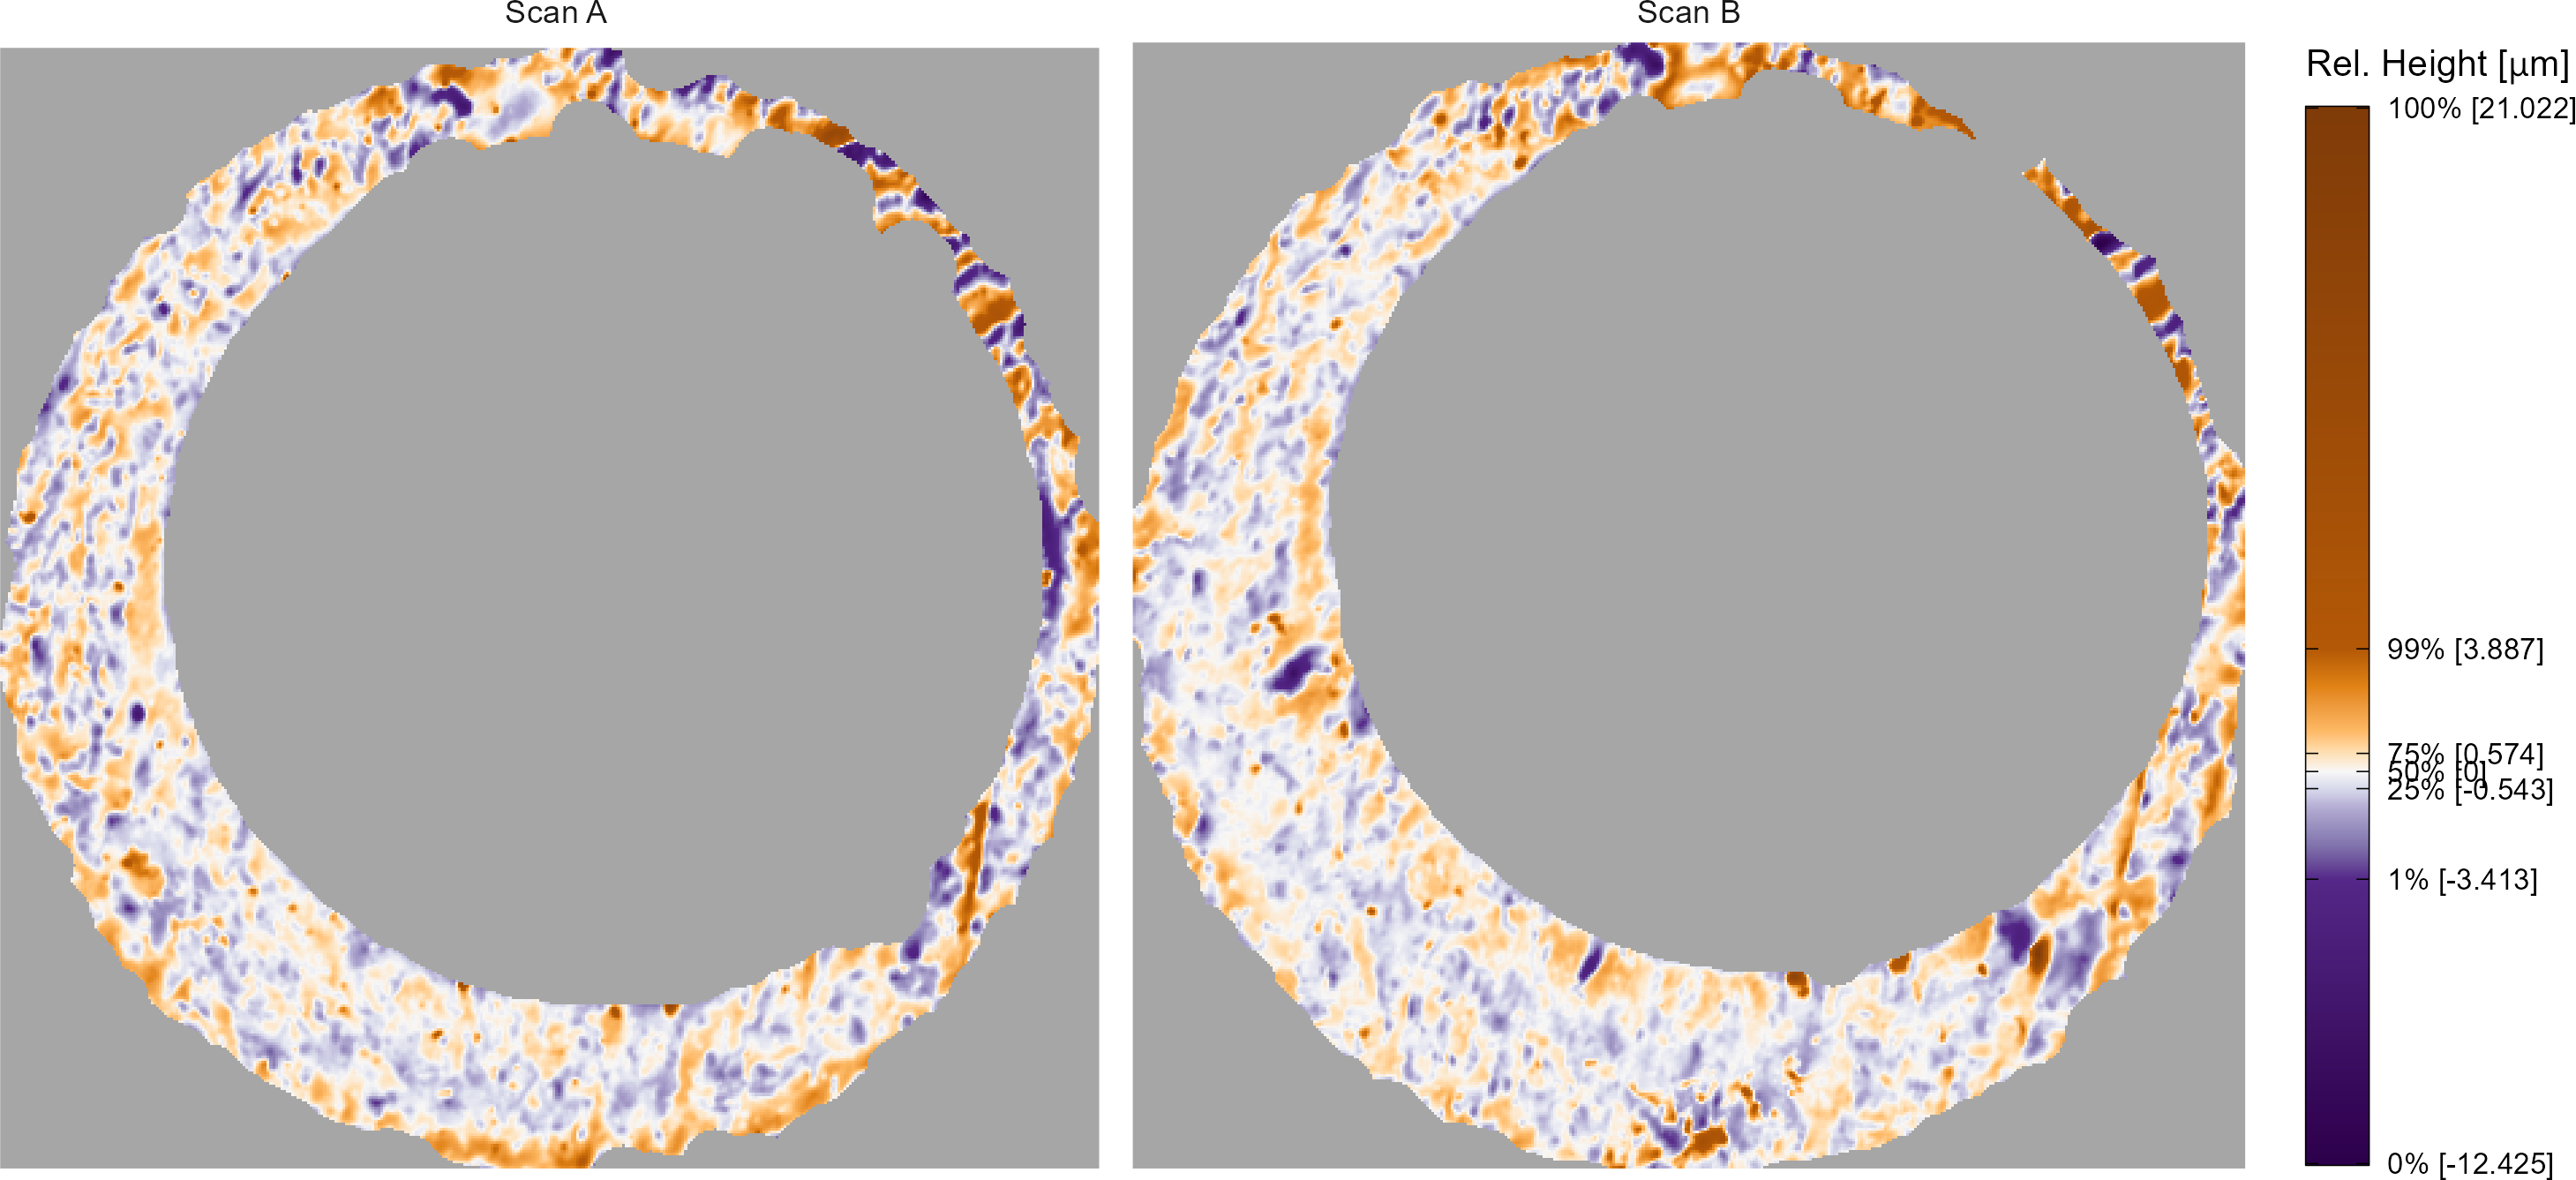
\includegraphics[width=.5\textwidth]{figures/matchPair} \caption{\label{fig:matchPair} A matching pair of processed cartridge case scans. We measure the similarity between these cartridge cases using the distinguishable breech face impressions on their surfaces.}\label{fig:unnamed-chunk-3}
\end{figure}

Note that the calculation of the CCF requires that all missing values,
including structural missing values, are imputed in \(A\) and \(B\). We
impute missing values in a scan with the average non-missing value in
that scan. As a result of imputing a large number of missing values, we
found in our experimentation the estimated registrations
\((\theta^*, m^*, n^*)\) to be reliable but the value of \(CCF_{\max}\)
to not be a reliable measure of similarity for scans. We discuss how we
compute more reliable measures of similarity in
\ref{featureCalculation}.

\hypertarget{full-scan-registration}{%
\subsubsection{Full-Scan Registration}\label{full-scan-registration}}

We first estimate the registration between two full scans \(A\) and
\(B\) using \autoref{alg:registration} with a rotation grid
\(\pmb{\Theta} = \{-30^\circ, -27^\circ,...,27^\circ,30^\circ\}\). This
results in an estimated registration \((m^*,n^*,\theta^*)\) and
similarity measure \(CCF_{\max}\). We also perform
\autoref{alg:registration} with the roles of \(A\) and \(B\) reversed,
meaning the target scan \(A\) is aligned to source scan \(B\).

To accommodate these two comparison directions, we introduce a new
subscript \(d = A,B\), referring to the source scan in
\autoref{alg:registration}. Consequently, we obtain two sets of
estimated registrations, \((m^*_d,n^*_d,\theta^*_d)\) and
\(CCF_{\max,d}\), for
\(d=A,B\).\footnote{In reality, the true aligning registrations in the two comparison directions are opposites of each other. However, because we compare discretely-indexed arrays using a nearest-neighbor interpolation scheme, the estimated registrations may differ slightly.}

\hypertarget{cell-based-registration}{%
\subsubsection{Cell-Based Registration}\label{cell-based-registration}}

We next perform a cell-based comparison procedure, which begins with
selecting one of the matrices, say \(A\), as the ``source'' matrix that
is partitioned into a grid of cells. The left side of
\autoref{fig:cellGridExample} shows an example of such a cell grid
overlaid on a scan. Each of these source cells will be compared to the
``target'' matrix, in this case \(B^*\). Because \(A\) and \(B^*\) are
already partially aligned from the full-scan registration procedure, we
compare each source cell to \(B^*\) using a new rotation grid of
\(\pmb{\Theta}'_A = \{\theta^*_A - 2^\circ, \theta^*_A - 1^\circ,\theta^*_A,\theta^*_A + 1^\circ,\theta^*_A + 2^\circ\}\).

We now extend the surface matrix notation introduced previously to
accommodate cells. Let \(A_{t}\) denote the \(t\)-th cell of matrix
\(A\), \(t = 1,...,T_A\) where \(T_A\) is the total number of cells
containing non-missing values in scan \(A\) (e.g., \(T_A = 43\) in
\autoref{fig:cellGridExample}) and let \((a_t)_{ij}\) denote the
\(i,j\)-th element of \(A_t\). The cell-based comparison procedure is
outlined in \autoref{alg:cellComparison}.

\begin{algorithm}[H]
\KwData{Source matrix $A$, target matrix $B^*$, grid size $R \times C$, and rotation grid $\pmb{\Theta}'_A$}
\KwResult{Estimated translations and $CCF_{\max}$ values per cell, per rotation}
Partition $A$ into a grid of $R \times C$ cells\;
Discard cells containing only missing values, leaving $T_A$ remaining cells\;
\For{$\theta \in \pmb{\Theta}'_A$}{
Rotate $B^*$ by $\theta$ to obtain $B^*_\theta$\;
\For{$t = 1,...,T_A$}{
Calculate $CCF_{\max, A,t,\theta} = \max_{m,n} (a_t \star b^*_\theta)_{mn}$\;
Calculate translation $[m^*_{A,t,\theta},n^*_{A,t,\theta}] = \arg \max_{m,n} (a_t \star b^*_\theta)_{mn}$
}
}
\Return{$\pmb{F}_A = \{(\theta, m^*_{A,t,\theta},n^*_{A,t,\theta}, CCF_{\max,A,t,\theta}) : \theta \in \pmb{\Theta}'_A, t = 1,...,T_A\}$}
\caption{Cell-Based Comparison Procedure}
\label{alg:cellComparison}
\end{algorithm}

We can think of \autoref{alg:registration} as a specific case of
\autoref{alg:cellComparison} where \(R = C = 1\), but we distinguish the
algorithms in this paper based on the intended use of the result. Rather
than exclusively returning the registration that maximizes the overall
CCF as in \autoref{alg:registration}, \autoref{alg:cellComparison}
returns the set \(\pmb{F}_A\) of translations and CCF values for each of
the \(T_A\) cells and each rotation in \(\pmb{\Theta}'_A\).

\begin{figure}[htbp]
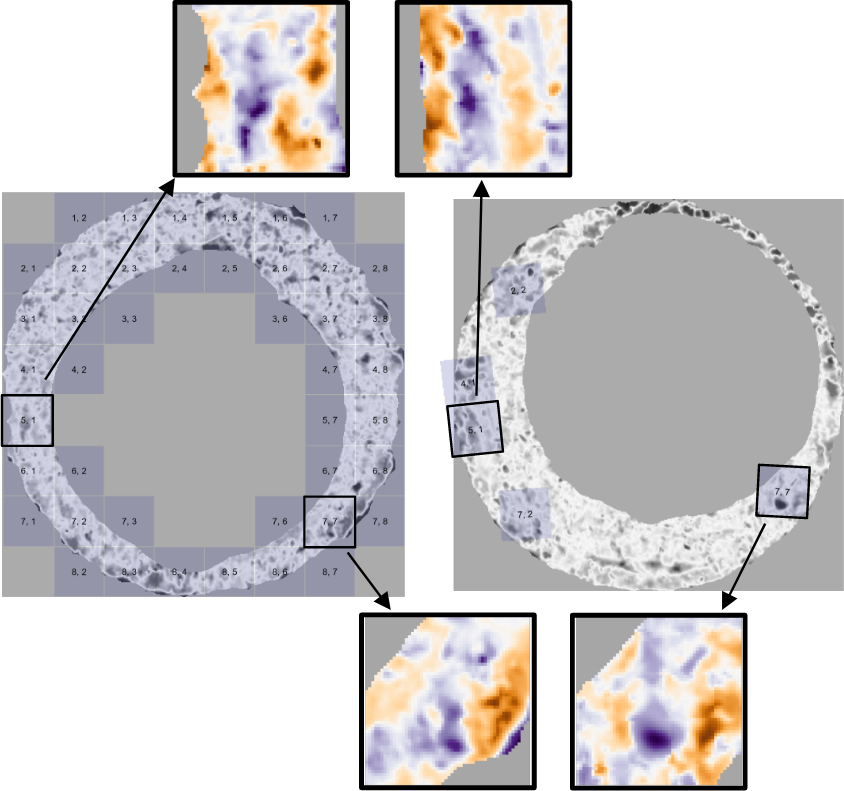
\includegraphics[width=.5\textwidth]{images/cellGridExample_nonMatch} \caption{\label{fig:cellGridExample} Estimated registrations of cells from a non-match pair of cartridge cases. A source scan (left) is separated into an $8 \times 8$ grid of cells. We exclude cells containing only missing values (visualized here as gray pixels). Each source cell is compared to a target scan (right) to estimate where it aligns best. We show a handful of cells at their estimated alignment in the target scan and magnify the surfaces captured by cell pairs 5, 1 and 7, 7. Although the cartridge case pair is non-matching, we note that there are similarities in the surface markings for these cell pairs.}\label{fig:unnamed-chunk-4}
\end{figure}

\autoref{fig:cellGridExample} shows the estimated registrations of cells
between two non-match cartridge cases. We magnify the surface values
captured by cell pairs 5, 1 and 7, 7 and note the similarities in the
surface values; for example, the dark purple region in the middle of the
cell 7, 7 pair.

Next, we introduce a set of similarity features for two cartridge case
scans. We calculate features at two scales: between two full scans and
between individual cells. Analogous to how a forensic examiner uses a
comparison microscope with different magnification levels, this allows
us to assess the similarity between two scans at the macro and micro
levels.

\hypertarget{featureCalculation}{%
\subsection{Feature Calculation}\label{featureCalculation}}

The result of the full scan and cell-based comparisons is a set of
estimated registrations with associated \(CCF_{\max}\) values. We
compute statistics on these results based on how we expect these
registrations to behave for matching vs.~non-matching cartridge case
pairs. Similar to the assumption made in the Congruent Matching Cells
algorithm, we expect that cells will agree on a particular registration
if the two cartridge cases truly match, suggesting that a measure of
spread of the estimated registrations would be an informative statistic.
Further, we would expect that the consensus-estimated registrations
should be approximately opposite across the two comparison directions
(i.e., registering \(A\) to \(B\) is the opposite of registering \(B\)
to \(A\)).

We first introduce a set of \emph{registration-based features} based on
descriptive statistics of the full scan and cell-based registrations.
Then, we discuss a set of \emph{density-based features} based on
applying a density-based clustering algorithm to the cell registrations
\(\pmb{F}_A\) and \(\pmb{F}_B\).

\hypertarget{registration-based-features}{%
\subsubsection{Registration-based
Features}\label{registration-based-features}}

For \(d = A\), we apply the registration transformation
\((m^*_A,n^*_A,\theta^*_A)\) to \(B\) to obtain \(B^*\). Because the
calculation of the \(CCF_{\max}\) requires imputing missing values in
both the source and target scans, we found the \(CCF_{\max}\) values to
not be a reliable measure of similarity for two cartridge cases.
Instead, we compute the \emph{pairwise-complete correlation}, \(cor\),
which is equivalent to the Pearson correlation between the overlapping,
non-missing elements of \(A\) and \(B^*\).

We compute the pairwise-complete correlation between \(A\) and \(B^*\),
resulting in \(cor_{\text{full},A}\). We repeat this in the other
comparison direction to obtain \(cor_{\text{full},B}\) and average the
two:
\(cor_{\text{full}} = \frac{1}{2}\left(cor_{A,\text{full}} + cor_{B,\text{full}}\right)\).
We assume that the \textbf{full-scan pairwise-complete correlation},
\(cor_{\text{full}}\), is large for truly matching cartridge cases.

Just as with the whole-scan registration, we calculate the
pairwise-complete correlation between each cell \(A_t\) and a matrix
\(B_{\theta,t}^*\) of the same size extracted from \(B^*_{\theta}\)
after translating by \([m^*_{A,\theta},n^*_{A,\theta}]\). From this we
obtain a set of pairwise-complete correlations for each cell and
rotation:
\(\{cor_{A,t,\theta} : t = 1,...,T_A, \theta \in \pmb{\Theta}'_A\}\).

We repeat \autoref{alg:cellComparison} and the pairwise-complete
correlation calculation using \(B\) as the source scan and \(A^*\) as
the target, resulting in cell-based registration set \(\pmb{F}_B\) and
pairwise-complete correlations
\(\{cor_{B,t,\theta} : t = 1,...,T_B, \theta \in \pmb{\Theta}'_B\}\).

For \(d = A,B\) and \(t = 1,...,T_d\), define the cell-wise maximum
pairwise-complete correlation as:

\[
cor_{d,t} = \max_{\theta} \{cor_{d,t,\theta} : \theta \in \pmb{\Theta}'_d\}.
\]

We compute two features, the \textbf{average} and \textbf{standard
deviation of the cell-based pairwise-complete correlations}, using the
correlation data:

\begin{align*}
\overline{cor}_{\text{cell}} &= \frac{1}{T_A + T_B} \sum_{d \in \{A,B\}} \sum_{t=1}^{T_d} cor_{d,t} \\
s_{cor} &= \sqrt{\frac{1}{T_A + T_B - 1} \sum_{d \in \{A,B\}} \sum_{t=1}^{T_d} (cor_{d,t} - \overline{cor}_{\text{cell}})^2}.
\end{align*}

We expect \(\overline{cor}_{\text{cell}}\) and \(s_{cor}\) to be large
for truly matching cartridge case pairs relative to non-matching pairs.

For \(d = A,B\) and \(t = 1,...,T_d\), define the per-cell estimated
translations and rotation as:

\begin{align*}
\theta^*_{d,t} &= \arg \max_{\theta} \{CCF_{\max,d,t,\theta} : \theta \in \pmb{\Theta}'_d\} \\
m^*_{d,t} &= m^*_{\theta^*_{d,t},d,t} \\
n^*_{d,t} &= n^*_{\theta^*_{d,t},d,t}.
\end{align*}

We compute the \textbf{standard deviation of the cell-based estimated
registrations} using the estimated translations and rotations:

\begin{align*}
s_{\theta^*} =  \sqrt{\frac{1}{T_A + T_B - 1} \sum_{d \in \{A,B\}} \sum_{t=1}^{T_d} (\theta^*_{d,t} - \bar{\theta}^*)^2} \\
s_{m^*} =  \sqrt{\frac{1}{T_A + T_B - 1} \sum_{d \in \{A,B\}} \sum_{t=1}^{T_d} (m^*_{d,t} - \bar{m}^*)^2} \\
s_{n^*} = \sqrt{\frac{1}{T_A + T_B - 1} \sum_{d \in \{A,B\}} \sum_{t=1}^{T_d} (n^*_{d,t} - \bar{n}^*)^2}
\end{align*}

where

\begin{align*}
\bar{m}^* &= \frac{1}{T_A + T_B} \sum_{d \in \{A,B\}}\sum_{t=1}^{T_d} m^*_{d,t} \\
\bar{n}^* &= \frac{1}{T_A + T_B} \sum_{d \in \{A,B\}} \sum_{t=1}^{T_d} n^*_{d,t} \\
\bar{\theta}^* &= \frac{1}{T_A + T_B} \sum_{d \in \{A,B\}} \sum_{t=1}^{T_d} \theta^*_{d,t}.
\end{align*}

We expect \(s_{\theta^*}, s_{m^*},s_{n^*}\) to be small for truly
matching cartridge case pairs relative to non-matching pairs.

\hypertarget{density-based-features}{%
\subsubsection{Density-Based Features}\label{density-based-features}}

We wish to identify when multiple cells agree on, or cluster around, a
particular registration value. However, pursuant with the notion that
only certain regions of matching cartridge cases contain distinctive
markings, it is unreasonable to assume and empirically rare that
\textbf{all} cells agree on a single registration. For example, the left
scatterplot in \autoref{fig:dbscanScatterplot} shows the per-cell
estimated translations \([m^*_{A,t,\theta}, n^*_{A,t,\theta}]\) when
scan \(A\) is used as source and \(B^*\) as target rotated by
\(\theta = 3^\circ\). The right scatterplot shows the per-cell estimated
translations with the roles of \(A\) and \(B^*\) reversed for
\(\theta = -3^\circ\). We see distinctive clusters, the black points, in
both plots among many noisy, gray points. The task is to isolate the
clusters among such noise.

We use the Density-Based Spatial Clustering of Applications with Noise
(DBSCAN) algorithm proposed by \citet{Ester1996} to identify clusters.
Compared to other clustering algorithms such as k-means
\citep{MacQueen1967}, DBSCAN does not require a pre-defined number of
expected clusters. Instead, the algorithm forms clusters if the number
of points within an \(\epsilon > 0\) distance of a point exceeds some
pre-defined threshold, \(minPts > 1\). If a point does not belong to a
cluster, then DBSCAN labels that point as ``noise.''

In \autoref{fig:dbscanScatterplot}, we use a \(4 \times 4\) grid of
cells to which we apply DBSCAN with \(\epsilon = 3\) and \(minPts = 3\).
The resulting clusters for the two comparison directions are 7 and 9
cells, respectively, visualized in \autoref{fig:dbscanScatterplot} as
black points. This indicates that about half of the cells in the
\(4 \times 4\) grid agree on a registration in both comparison
directions. Additionally, the mean cluster centers are approximately
close to 0:
\((\hat{m}_A,\hat{n}_A,\hat{\theta}_A) \approx (0.29, 0.57, 0^\circ)\)
when \(A\) is used as source compared to
\((\hat{m}_B,\hat{n}_B,\hat{\theta}_B) \approx (-0.67, 0.00, 0^\circ)\)
when \(B^*\) is used as source. If \(A\) and \(B\) were truly matching
and the full scan registration from \autoref{alg:registration}
successfully aligned the two scans, then we wouldn't expect the cells to
move much in their respective registrations, which is illustrated in
this example. For non-matching scans, we wouldn't expect the cell
registrations to agree only by coincidence.

\begin{figure}[htbp]
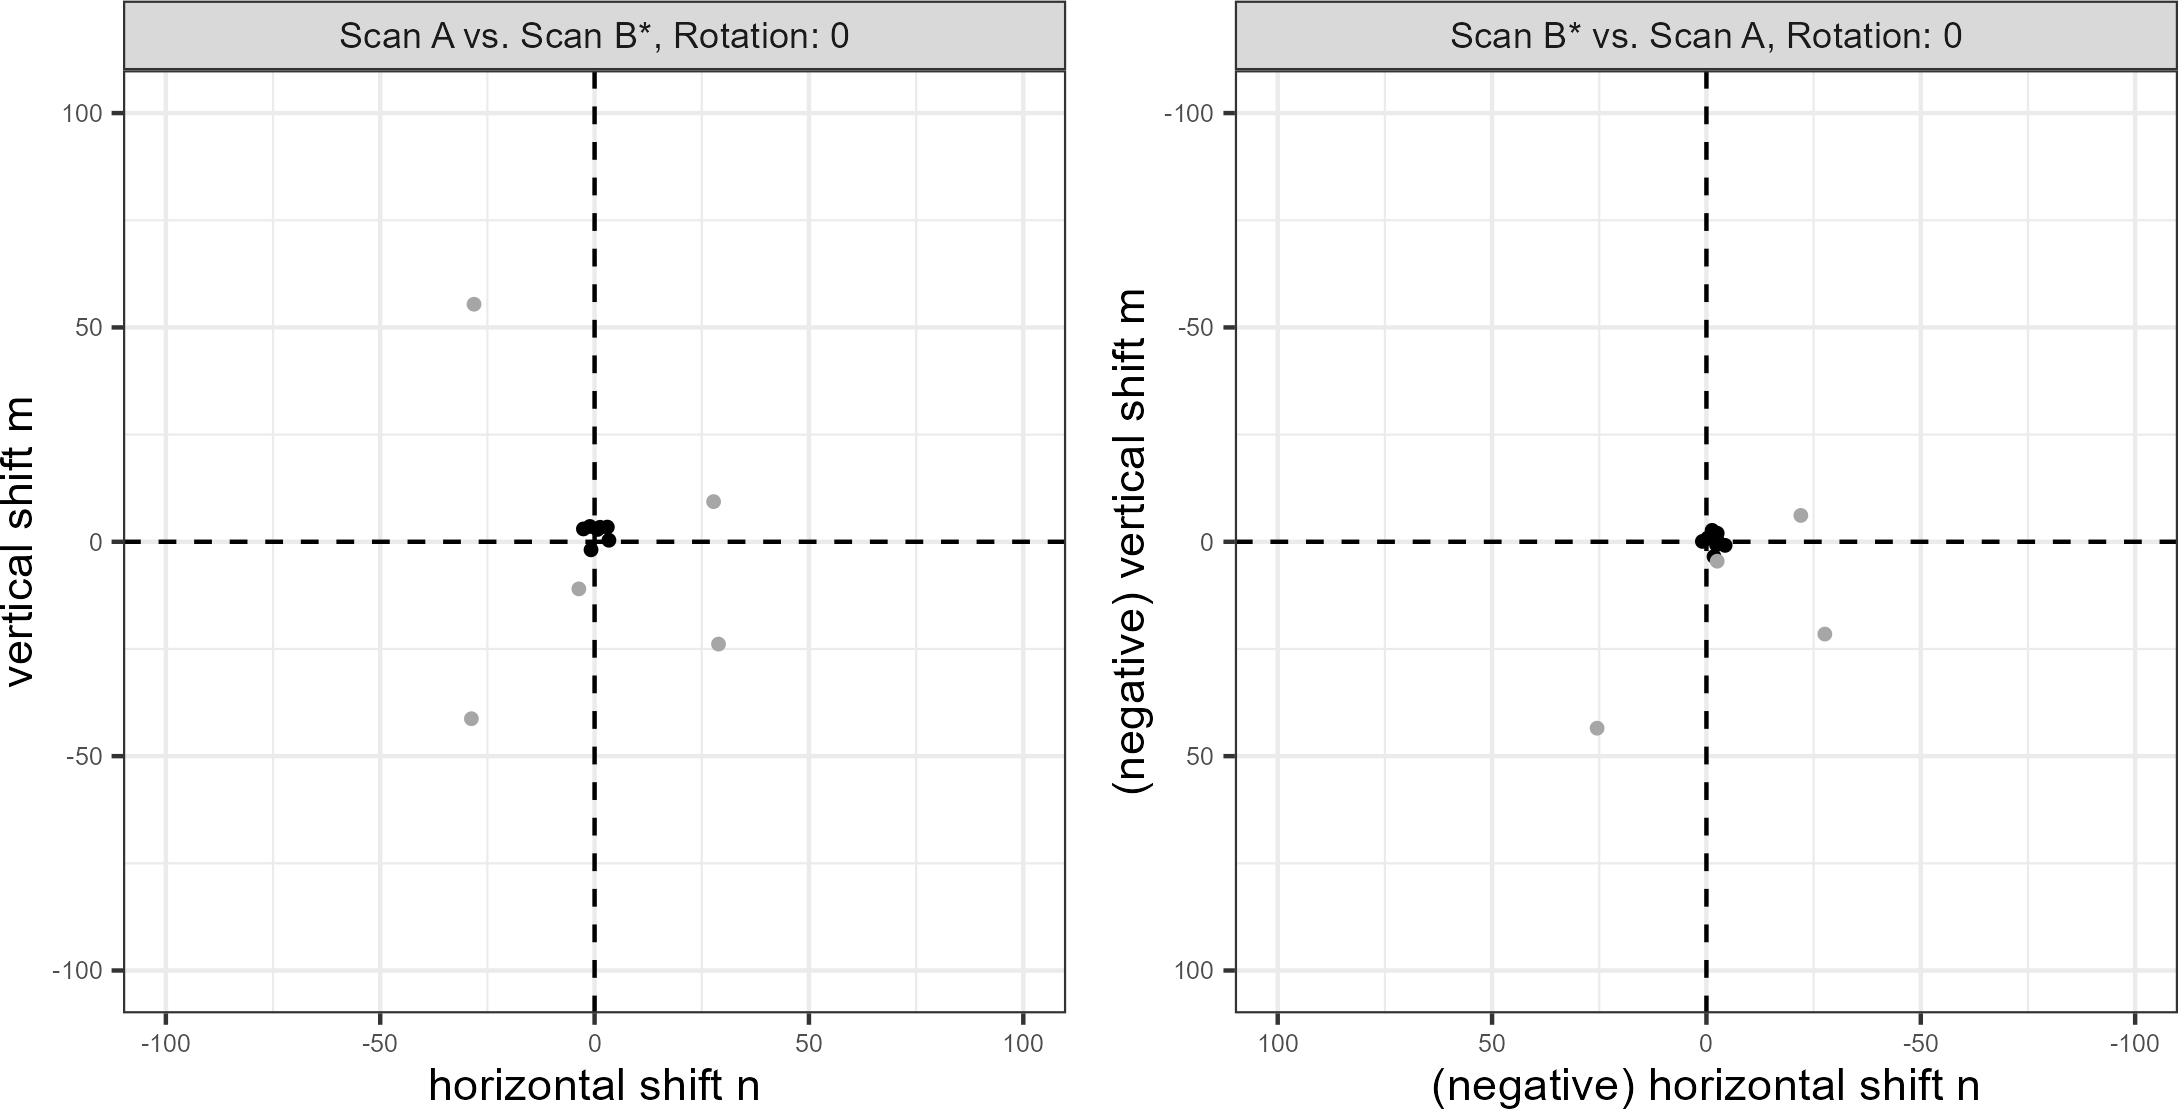
\includegraphics[width=.5\textwidth]{figures/dbscanScatterplot} \caption{\label{fig:dbscanScatterplot} Cluster assignments based on the Density Based Spatial Clustering with Applications to Noise (DBSCAN) algorithm for estimated translations in two comparison directions. Clustered points are shown as black while "noise" points are gray. We see that the clusters are both centered near the origin, indicating no further transformation is needed. Points are jittered for visibility.}\label{fig:unnamed-chunk-7}
\end{figure}

To calculate the density-based features, we first use a 2D kernel
density estimator \citep{MASS} to identify the rotation
\(\hat{\theta}_d\) at which the per-cell translations achieve the
highest density. Next, we compute clusters using the DBSCAN algorithm
amongst the estimated translations
\(\{(m^*_{d,t,\hat{\theta}_d},n^*_{d,t,\hat{\theta}_d}) : t = 1,...,T_d\}\)
like those shown in \autoref{fig:dbscanScatterplot}.\footnote{If more
  than one cluster is identified, we binarize the points based on
  whether they were assigned to any cluster or if they are a noise point
  and proceed as if there is only one cluster. We assume that two or
  more clusters form only because of the course rotation grid
  considered. Were a finer grid used, the points would coalesce into a
  single cluster around the true translation value. This assumption has
  empirical support through our experimentation.} Let \(\pmb{C}_d\)
denote the set of cells in the DBSCAN cluster. We treat the mean cluster
centers as the estimated translations \([\hat{m}_d,\hat{n}_d]\).

We calculate four features from the density-based clustering procedure:
\textbf{average DBSCAN cluster size} \(C\), the \textbf{DBSCAN cluster
indicator} \(C_0\), and the \textbf{root sum of squares of the
dens}ity-estimated registrations
\((\Delta_\theta, \Delta_{\text{trans}})\) defined as:

\begin{align*}
C &= \frac{1}{2}\left(|\pmb{C}_A| + |\pmb{C}_B|\right) \\
C_0 &= I(|\pmb{C}_A| > 0 \text{ and } |\pmb{C}_B| > 0)\\
\Delta_\theta &= |\hat{\theta}_A + \hat{\theta}_B| \\
\Delta_{\text{trans}} &= \sqrt{(\hat{m}_A + \hat{m}_B)^2 + (\hat{n}_A + \hat{n}_B)^2}
\end{align*} where \(|\pmb{C}_d|\) denotes the cardinality of
\(\pmb{C}_d\) and \(I(\cdot)\) is the identity function equal to 1 if
the predicate argument ``\(\cdot\)'' evaluates to TRUE and 0 otherwise.
We use both \(C\) and \(C_0\) because of potential missingness in the
values of \(C\) if no cluster is identified. Missing \(C\) values are
imputed using the median non-missing value when fitting classifiers, so
the missingness information is retained in \(C_0\).

For truly matching cartridge case pairs, we expect \(C\) to be large and
\(\Delta_\theta, \Delta_{\text{trans}}\) to be small relative to
non-matching pairs and for \(C_0\) to be equal to 1.

In summary, there are 10 total features, 6 registration-based and 4
density-based, that we calculate for each cartridge case pair. We list
the 10 features in \autoref{tab:allFeatures}. In the next section, we
discuss how we use these features in a model-based approach to obtain
similarity scores.

\begin{table}[htbp]
\centering
\begin{tabular}{p{.4\linewidth}p{.59\linewidth}}
$cor_{\text{full}} \in [0,1]$ & Full-scan pairwise-complete correlation \\
$\overline{cor}_{\text{cell}} \in [0,1]$ & Average cell-based pairwise-complete correlation \\
$s_{cor} \in [0,\infty)$ & Standard deviation of the cell-based pairwise-complete correlations \\
$s_{m^*} \in [0,\infty)$ & Standard deviation of the cell-based vertical translations (in microns) \\
$s_{n^*} \in [0,\infty)$ & Standard deviation of the cell-based horizontal translations (in microns) \\
$s_{\theta^*} \in [0,\infty)$ & Standard deviation of the cell-based rotations (degrees) \\
$C \in \{minPts,...,T_S\}$ & Average DBSCAN cluster size (for scan $S$)\\
$C_0 \in \{0,1\}$ & DBSCAN cluster indicator \\
$\Delta_\theta \in [0^\circ,180^\circ)$ & Absolute sum of the density-estimated rotations (degrees) \\
$\Delta_{\text{trans}} \in [0,\infty)$ & Root sum of squares of the density-estimated translations (in microns)
\end{tabular}
\caption{Ten features we compute for each cartridge case pair.}
\label{tab:allFeatures}
\end{table}

\hypertarget{model-fitting}{%
\subsection{Model Fitting}\label{model-fitting}}

We use a data set of 510 cartridge cases scanned from 25 firearms. We
randomly split the data into 10 firearms for training and 15 firearms
for testing. This resulted in a training data set of 210 cartridge
cases, \(\binom{210}{2} = 21,945\) pairwise comparisons, and a testing
set of 300 cartridge cases, \(\binom{300}{2} = 44,850\) pairwise
comparisons. Because we consider every pairwise comparison between these
scans, there is a relatively large class imbalance between matches and
non-matches in these data sets. Specifically, non-matching comparisons
make up 19,756 of the 21,945 (90.0\%) training comparisons and 41,769 of
the 44,850 (93.1\%) testing comparisons.

We use 10-fold cross-validation repeated thrice \citep{caret} to train
two binary classifiers based on a logistic regression and a random
forest \citep{breiman, randomForest}. These models predict the
probability that a pair of cartridge cases match (the \emph{match
probability}). Then, the model classifies the pair as a match or
non-match depending on whether the match probability exceeds a set
threshold.

Models trained to maximize accuracy on imbalanced data often exhibit a
``preference'' for classifying new observations as the majority class
\citep{Fernndez2018}, which in our case are non-matches. To address this
imbalance, we explore three possible subsampling techniques:
\emph{upsampling} the number of match comparisons to equal the number of
non-match comparisons, \emph{downsampling} the number of non-match
comparisons to equal the number of match comparisons, and performing no
subsampling.

An optimization criterion commonly used for imbalanced data is to select
the model that maximizes the area under the Receiver Operating
Characteristic (ROC) curve, which measures the performance of a model
under different threshold values \citep{James2013}. The model that
maximizes this area, commonly abbreviated AUC, is one that performs best
under a variety of threshold values relative to the other models - this
consistency is a desired trait. Using the ROC curve, we choose the match
probability threshold that balances the true negative and true positive
(equivalently, the false positive and false negative) rates on the
training data.

We optimize the models by performing a grid search across the following
parameters:

\begin{itemize}
\item
  DBSCAN parameters \(\epsilon \in \{3,4,...,15\}\) and
  \(minPts \in \{3,4,...,10\}\),
\item
  Subsampling technique: downsampling, upsamplng, and no subsampling,
\item
  For the random forest, the ``mtry'' variable, which controls the
  number of candidate variables a decision tree has available at each
  split \citep{breiman}, and
\item
  Match probability, \(p \in [0,1]\)
\end{itemize}

Once we have a trained model, we use it to predict the match probability
and classify a new cartridge case pair. We use this match probability as
a similarity score where larger values correspond with more similar
cartridge cases. We compute this score for the pairwise comparisons in
the test data as a means of comparing the generalizability of the
various models. The following section details the results of this
cross-validation training/testing procedure. We refer the reader to
\url{https://github.com/jzemmels/rules_vs_scores} for the source code
used to derive these results.

\hypertarget{results}{%
\section{Results}\label{results}}

\hypertarget{roc-curves}{%
\subsection{ROC Curves}\label{roc-curves}}

First, we consider results from the training procedure.
\autoref{fig:rocPlot} shows the resulting ROC curves for three
classifiers trained on the training data set. For comparison to the
logistic regression (LR) and random forest (RF) classifiers, we also
consider a classifier based on the Congruent Matching Cells (CMC) method
proposed in \citet{song_proposed_2013}. We obtained these CMC results
using the implementation available in the \texttt{cmcR} R package
\citep{cmcR} and the same training and testing set. Similar to the two
statistical models, we chose CMC method parameters using the AUC as an
optimization criterion. We note that the interpretation of the
thresholds used for the LR and RF models, which classify a pair as a
match if its predicted class probability exceeds a threshold, differ
from that of the CMC method, which classifies a pair as a match if its
associated CMC count exceeds a threshold.

The ROC curves allow us to visually compare the behavior of these three
classifiers under various score thresholds where curves closer to the
top-left corner are preferred. The LR and RF models perform comparably
as evidenced by the similar curves on the right side of
\autoref{fig:rocPlot}. The left side shows a zoomed-in version of the
top left corner of plot, where we are more easily able to identify the
superior performance of random forest model. The CMC method performs
comparably worse as evidenced by the noticeably lower ROC curve.

To numerically compare the three classifiers, we compute the area under
the ROC curve (AUC) as well as the score threshold (Thresh.) that
balances the false negative and false positive rates (the equal error
rate or EER). The AUC for logistic regression and random forest
classifiers are much higher than the AUC of the CMC method classifier.
Each model has a different score threshold that yields the equal error
rate, which we visualize as points along the three ROC curves in
\autoref{fig:rocPlot}. We use these thresholds to compute both the
training and test classification results summarized below. We see that
the random forest classifier has the lowest equal error rate out of the
three models with the logistic regression classifier a close second.

\begin{figure*}[htbp]

{\centering 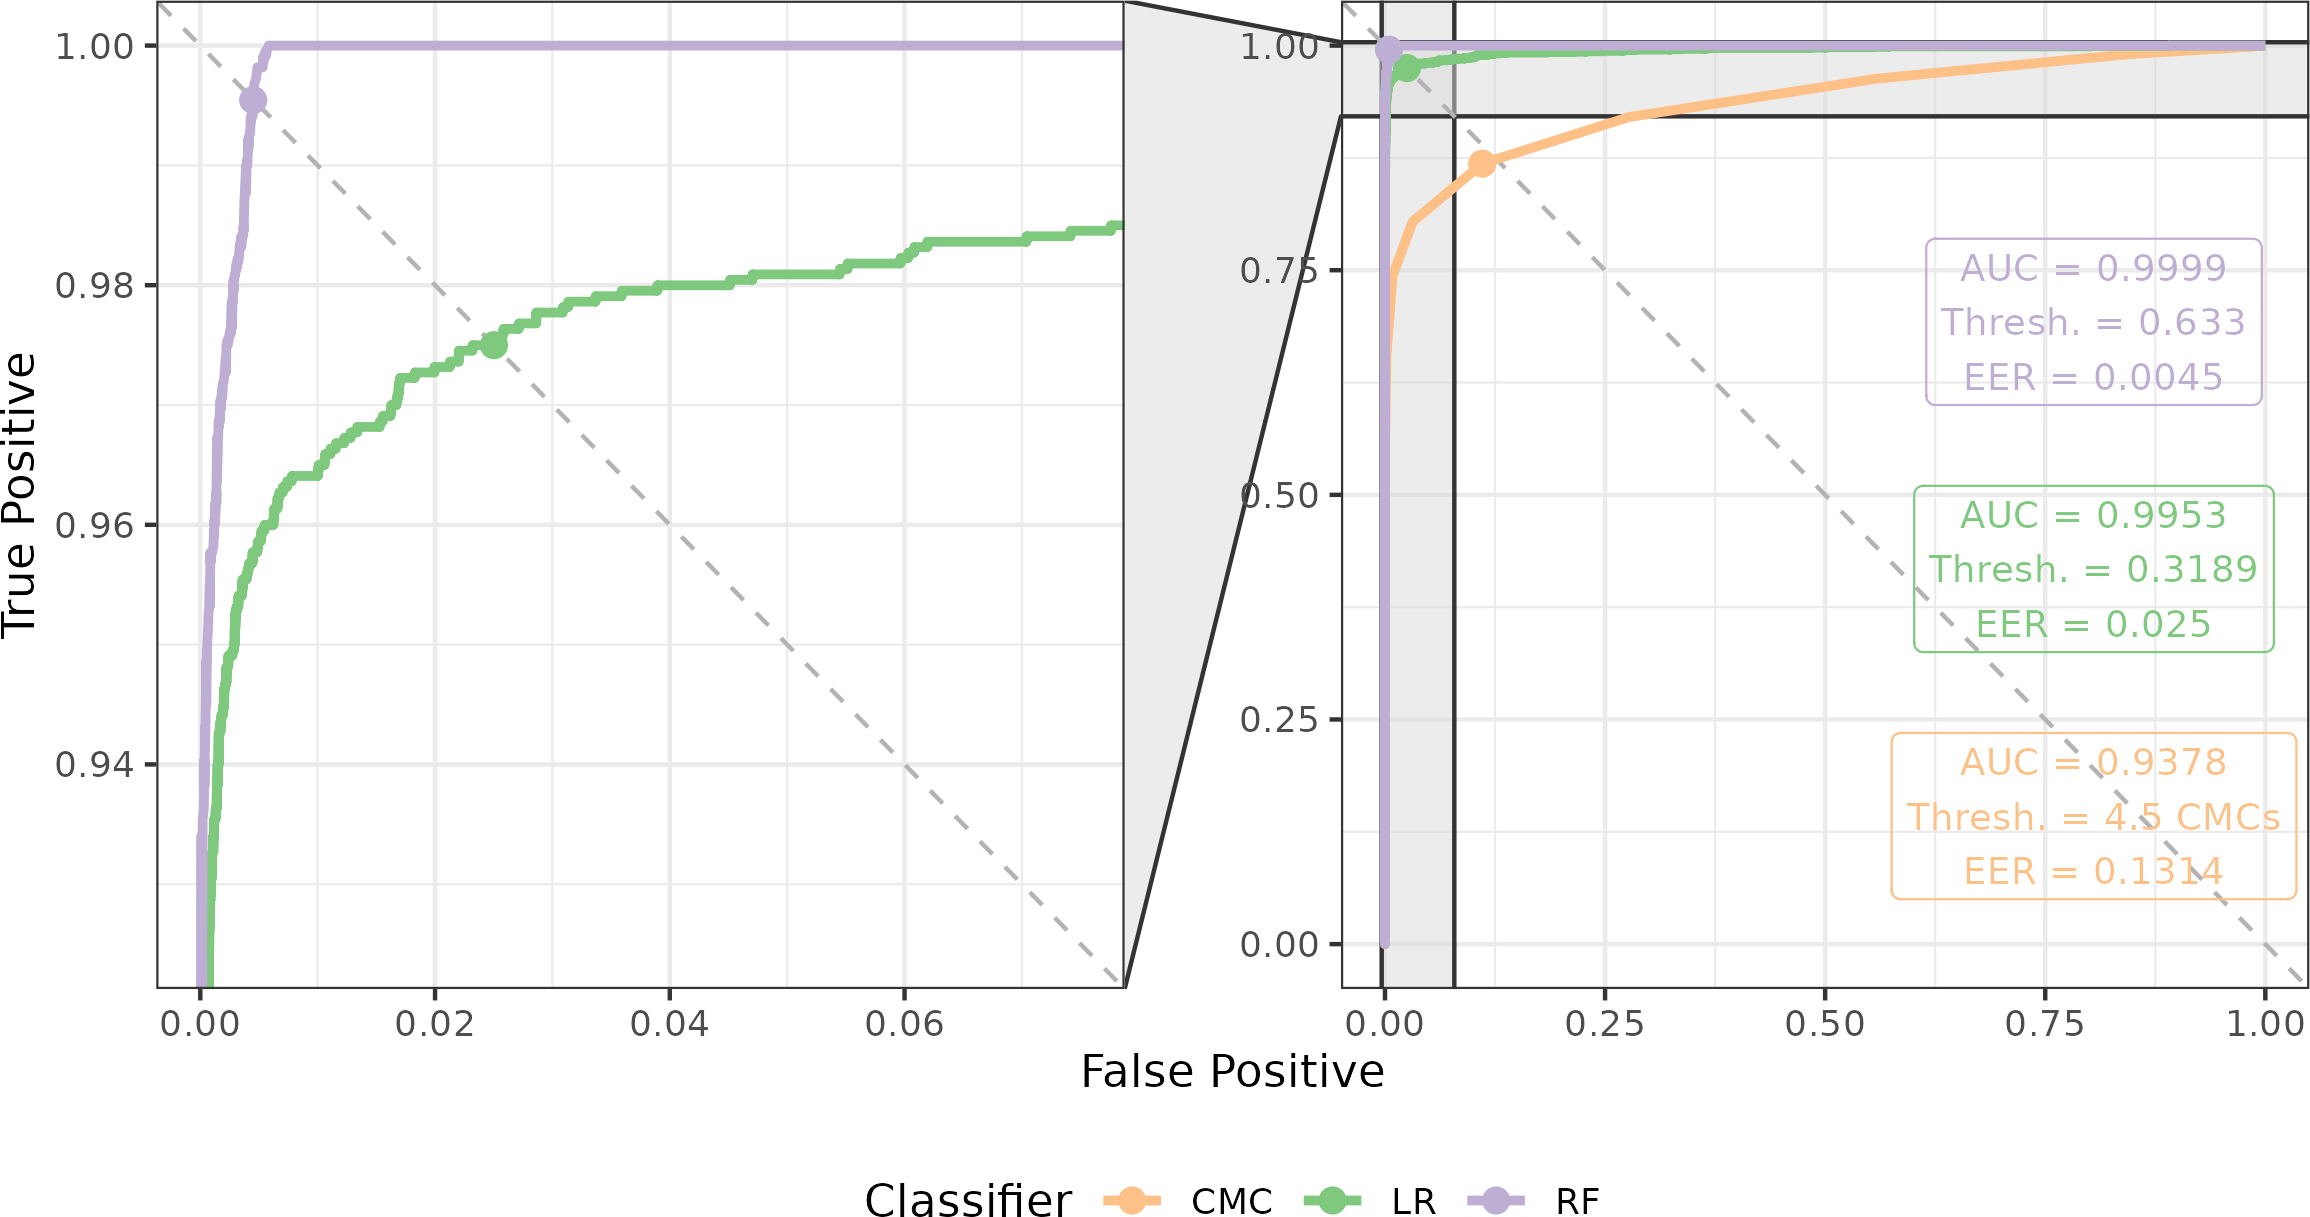
\includegraphics[width=\textwidth]{images/resultsPlots/rocPlot} 

}

\caption{ROC curves for logistic regression (LR), random forest (RF), and Congruent Matching Cells classifiers. On the left, we zoom into the top-left corner of the ROC curve plot to better distinguish between the LR and RF curves. We see that the two statistical model classifiers have higher area under the curve (AUC) and lower equal error rate (EER) values than the CMC method. We also show the score classification cutoffs (Thresh.) used for each of the four models to achieve the equal error rate values.}\label{fig:rocPlot}
\end{figure*}

\hypertarget{optimized-model-comparison}{%
\subsection{Optimized Model
Comparison}\label{optimized-model-comparison}}

\autoref{fig:trainTestAccuracy} summarizes the training and testing
accuracy, true negative and true positive rates for four binary
classifiers. Three of the four classifiers are associated with the equal
error rate points shown in \autoref{fig:rocPlot}. The fourth classifier
is based on a simple, binary decision rule that classifies a pair as a
match if the DBSCAN algorithm identifies a cluster in the cell-wise
estimated registrations (in \emph{both} comparison directions) and as a
non-match otherwise. This is analogous to the decision rule proposed in
\citet{zhang_convergence_2021}. We optimized this ``Cluster Indicator''
classifier by selecting DBSCAN parameters that balanced the train true
positive and true negative rates, resulting in parameters
\(\epsilon = 15\) and \(minPts = 8\). We refer to the Cluster Ind. and
CMC-based classifiers as ``rule-based'' because the fundamental
similarity scoring and decision-making mechanisms are based on one or
more binary rules. Comparatively, the ``model-based'' logistic
regression and random forest classifiers rely on a learned mapping of
the numerical features summarized in \autoref{tab:allFeatures} to a
continuous class probability that is ultimately used to discriminate
between match and non-match comparisons.

In \autoref{fig:trainTestAccuracy}, we distinguish between the training
and testing results using gray and black points/line segments,
respectively, which allows us to assess the generalizability of the
various models to new comparisons. The conclusions drawn from
\autoref{fig:trainTestAccuracy} are intended to primarily be qualitative
and comparative across models. \autoref{tab:trainDataResults} and
\autoref{tab:testDataResults} in the Appendix provide a numerical
summary of these results.

\begin{figure*}[htbp]

{\centering 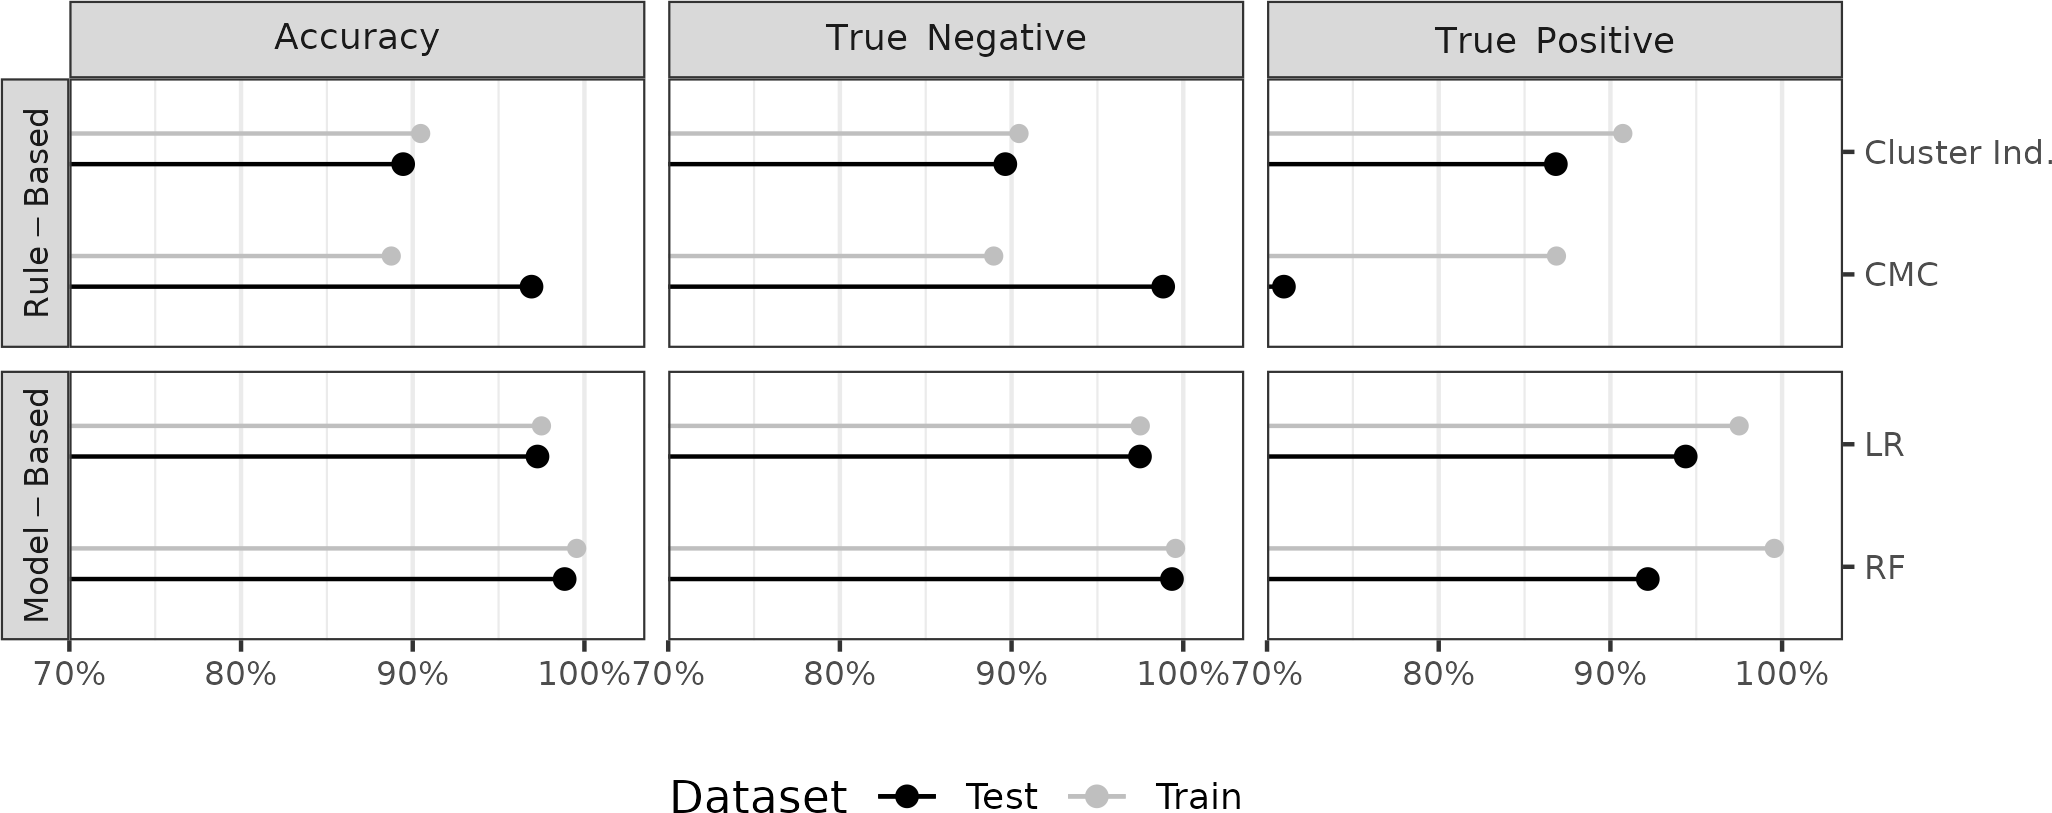
\includegraphics[width=\textwidth]{images/resultsPlots/classifResultsPlt_trainTest} 

}

\caption{\label{fig:trainTestAccuracy} We summarize classification accuracy, true negative, and true positive rates for both the training and testing results, represented as gray and black points/lines respectively, for four binary classifiers. Our primary interest is the test data results, but visualizing the training data results allows us to assess the generalizability of the classifiers after training. The first row summarizes results from a decision rule classifier based on whether the DBSCAN algorithm identifies a cluster among a comparison's cell-wise registrations. The second row summarizes results from a classifier based on the Congruent Matching Cells method. The third and fourth rows show results from training/testing classifiers based on a random forest (RF) and logistic regression (LR).}\label{fig:unnamed-chunk-9}
\end{figure*}

We first compare the training and testing results across the four models
and three columns in \autoref{fig:trainTestAccuracy}. In general, the
true negative rates based on the test data are slightly lower than those
of the training data, with the exception of the CMC method that has a
considerably higher test true negative rate, indicating that the models'
ability to distinguish between non-matching comparisons generalizes well
to the testing data. In contrast, the true positive rates tend to be
lower for the test data compared to the training data across the various
models, which indicates a potential difference between the training and
testing match comparisons. As we discuss below, there is a single
firearm among the 15 test firearms that contributes the majority of
false negative (misclassified match) test classifications. Despite lower
true positive rates, the overall accuracy between the training and
testing sets are comparable because of the large class imbalance between
matching and non-matching comparisons in both.

In general, we see that the logistic regression (LR) and random forest
(RF) models perform comparable to each other in accuracy, true negative,
and true positive rates. If we compare the ``\(C_0\) +
Registration''-trained models in the second vs.~the ``All ACES''-trained
models in the third row, we see that the addition of the other ACES
features leads to improved test true negative and true positive rates
(and consequently overall accuracy) with the most noticeable gains
observed in the true positive rate. Across the four models, the random
forest classifier has the largest overall test accuracy and true
negative rates of 98.9\% and 99.3\%, respectively. The logistic
regression classifier has the largest overall true positive rate of
94.4\% (see \autoref{tab:testDataResults} for more details).

\hypertarget{similarity-score-investigation}{%
\subsection{Similarity Score
Investigation}\label{similarity-score-investigation}}

While it's useful to consider the accuracy, true negative, and true
positive rates to compare various models, forensic examiners would
likely not use the binary classification returned by a classifier in
casework. Instead, they would consider the match probability predicted
by the model as a similarity score and incorporate it into their
decision-making process. As such, we also consider the distribution of
the predicted similarity scores for matching and non-matching
comparisons. \autoref{fig:testProbs} shows a dot plot of the predicted
similarity scores for the 41,769 non-match and 3,181 match comparisons
in the test set. Specifically, these probabilities are predicted by the
logistic regression model represented in
\autoref{fig:trainTestAccuracy}. As we expect, few non-match comparisons
have large similarity scores, which justifies the high true negative
rate for the model-based classifiers observed in
\autoref{fig:trainTestAccuracy}. However, there is a surprising number
of matching comparisons that have a low match probability.

\begin{figure}[htbp]

{\centering 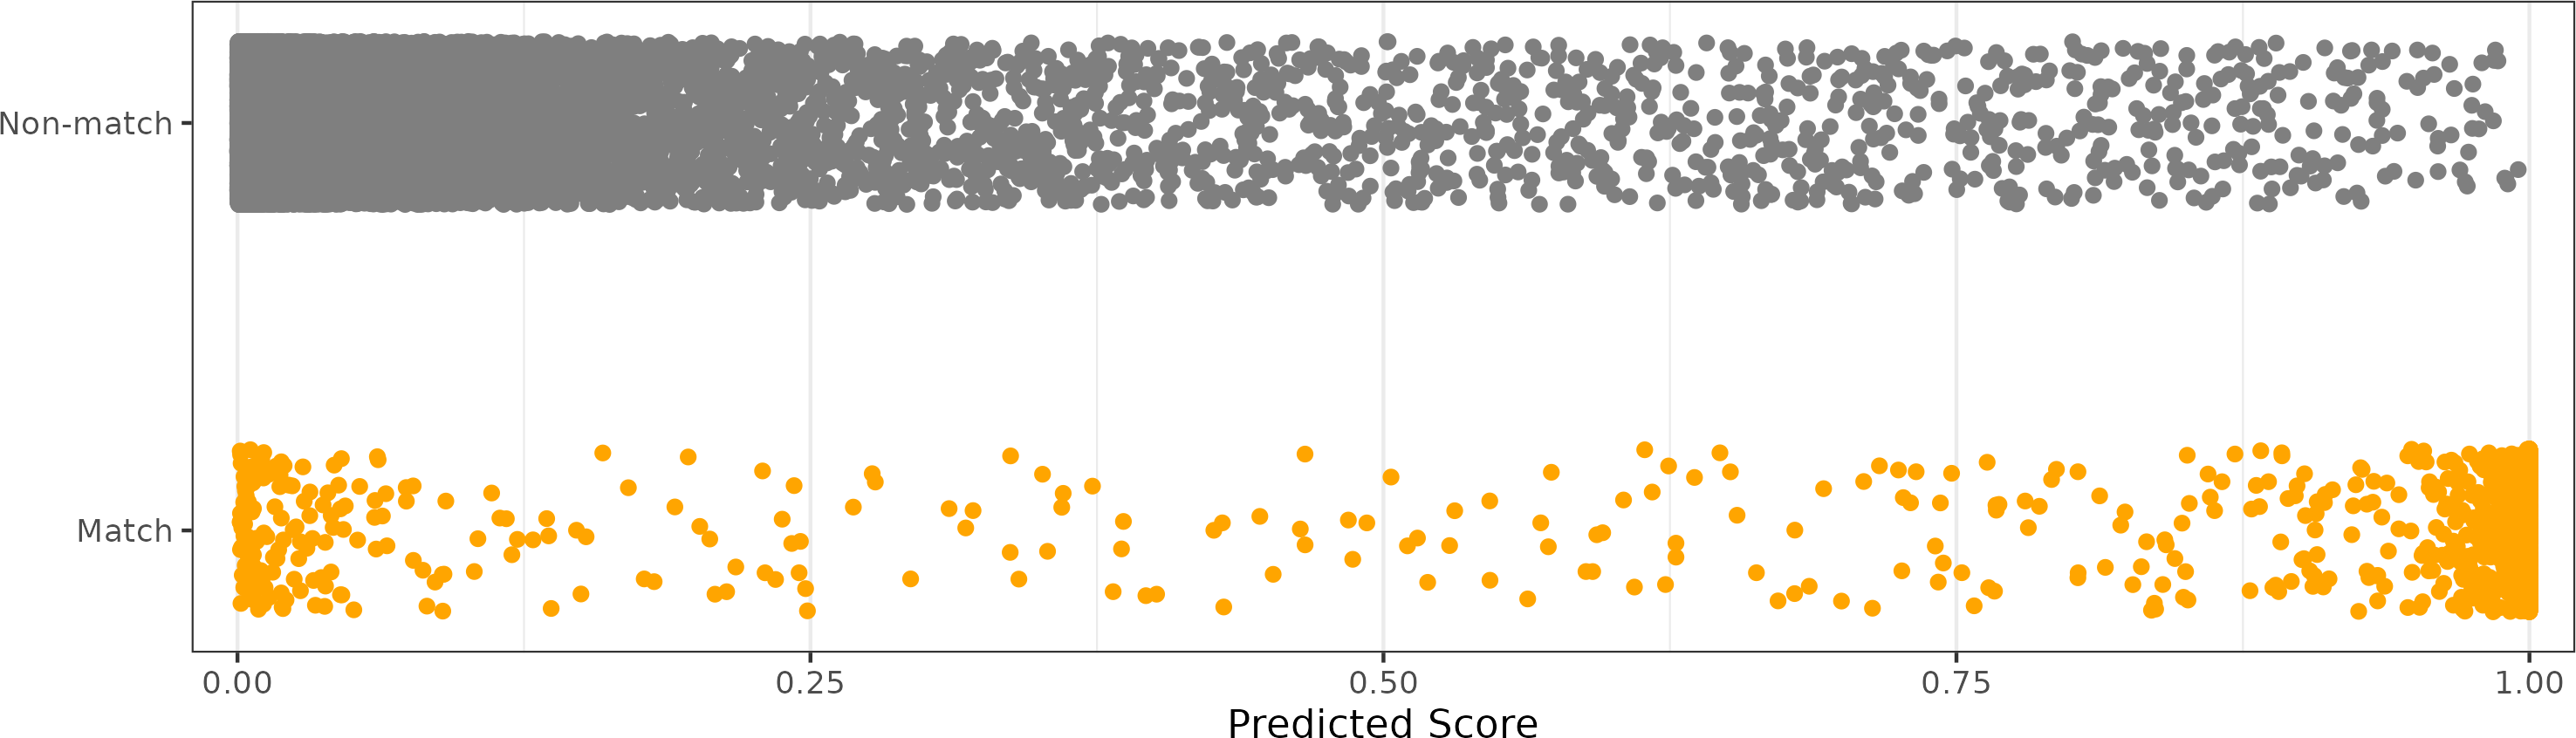
\includegraphics[width=.5\textwidth]{images/resultsPlots/testProbs_plt} 

}

\caption{\label{fig:testProbs} A dot plot of the predicted similarity scores for the non-match and match comparisons in the test set based on a logistic regression model. As we expect, the non-match comparisons tend to have a low match probability. However, we see that there are many matching comparisons that have a low match probability.}\label{fig:unnamed-chunk-10}
\end{figure}

To explain the matching comparisons with low similarity scores, we
visualize in \autoref{fig:testProbs-byFirearm} the predicted similarity
scores for matching test comparisons distinguished by the 15 test
firearm ID. We see that the firearm T has far more matching comparisons
with low similarity scores compared to the other 14 test firearms. This
is further underscored by the right side of the
\autoref{fig:testProbs-byFirearm}, which shows the ratio of
misclassifications to total comparisons for every pair of test firearms
based on the same logistic regression model used in
\autoref{fig:testProbs}. The main diagonal shows the false negative
misclassifications while the off-diagonal shows the false positives. We
use blank tiles for comparisons where 0 misclassifications occurred. We
see that the false negative rate for firearm T of 37\% is far greater
than that of other firearm pairs. The 130 false negative firearm T
comparisons comprise 75\% of all 173 false negative test comparisons and
about 4\% of all 3,181 matching test comparisons. In sum, the model
performs distinctly worse at identifying matching comparisons from
firearm T compared to the other firearms, which partially explains the
lower test true positive rates noted in \autoref{fig:trainTestAccuracy}.
Anecdotally, upon visual inspection of the scans from firearm T, we
noted a lack of consistent markings on their surfaces, which isn't the
case for scans from other test firearms.

\begin{figure*}[htbp]

{\centering 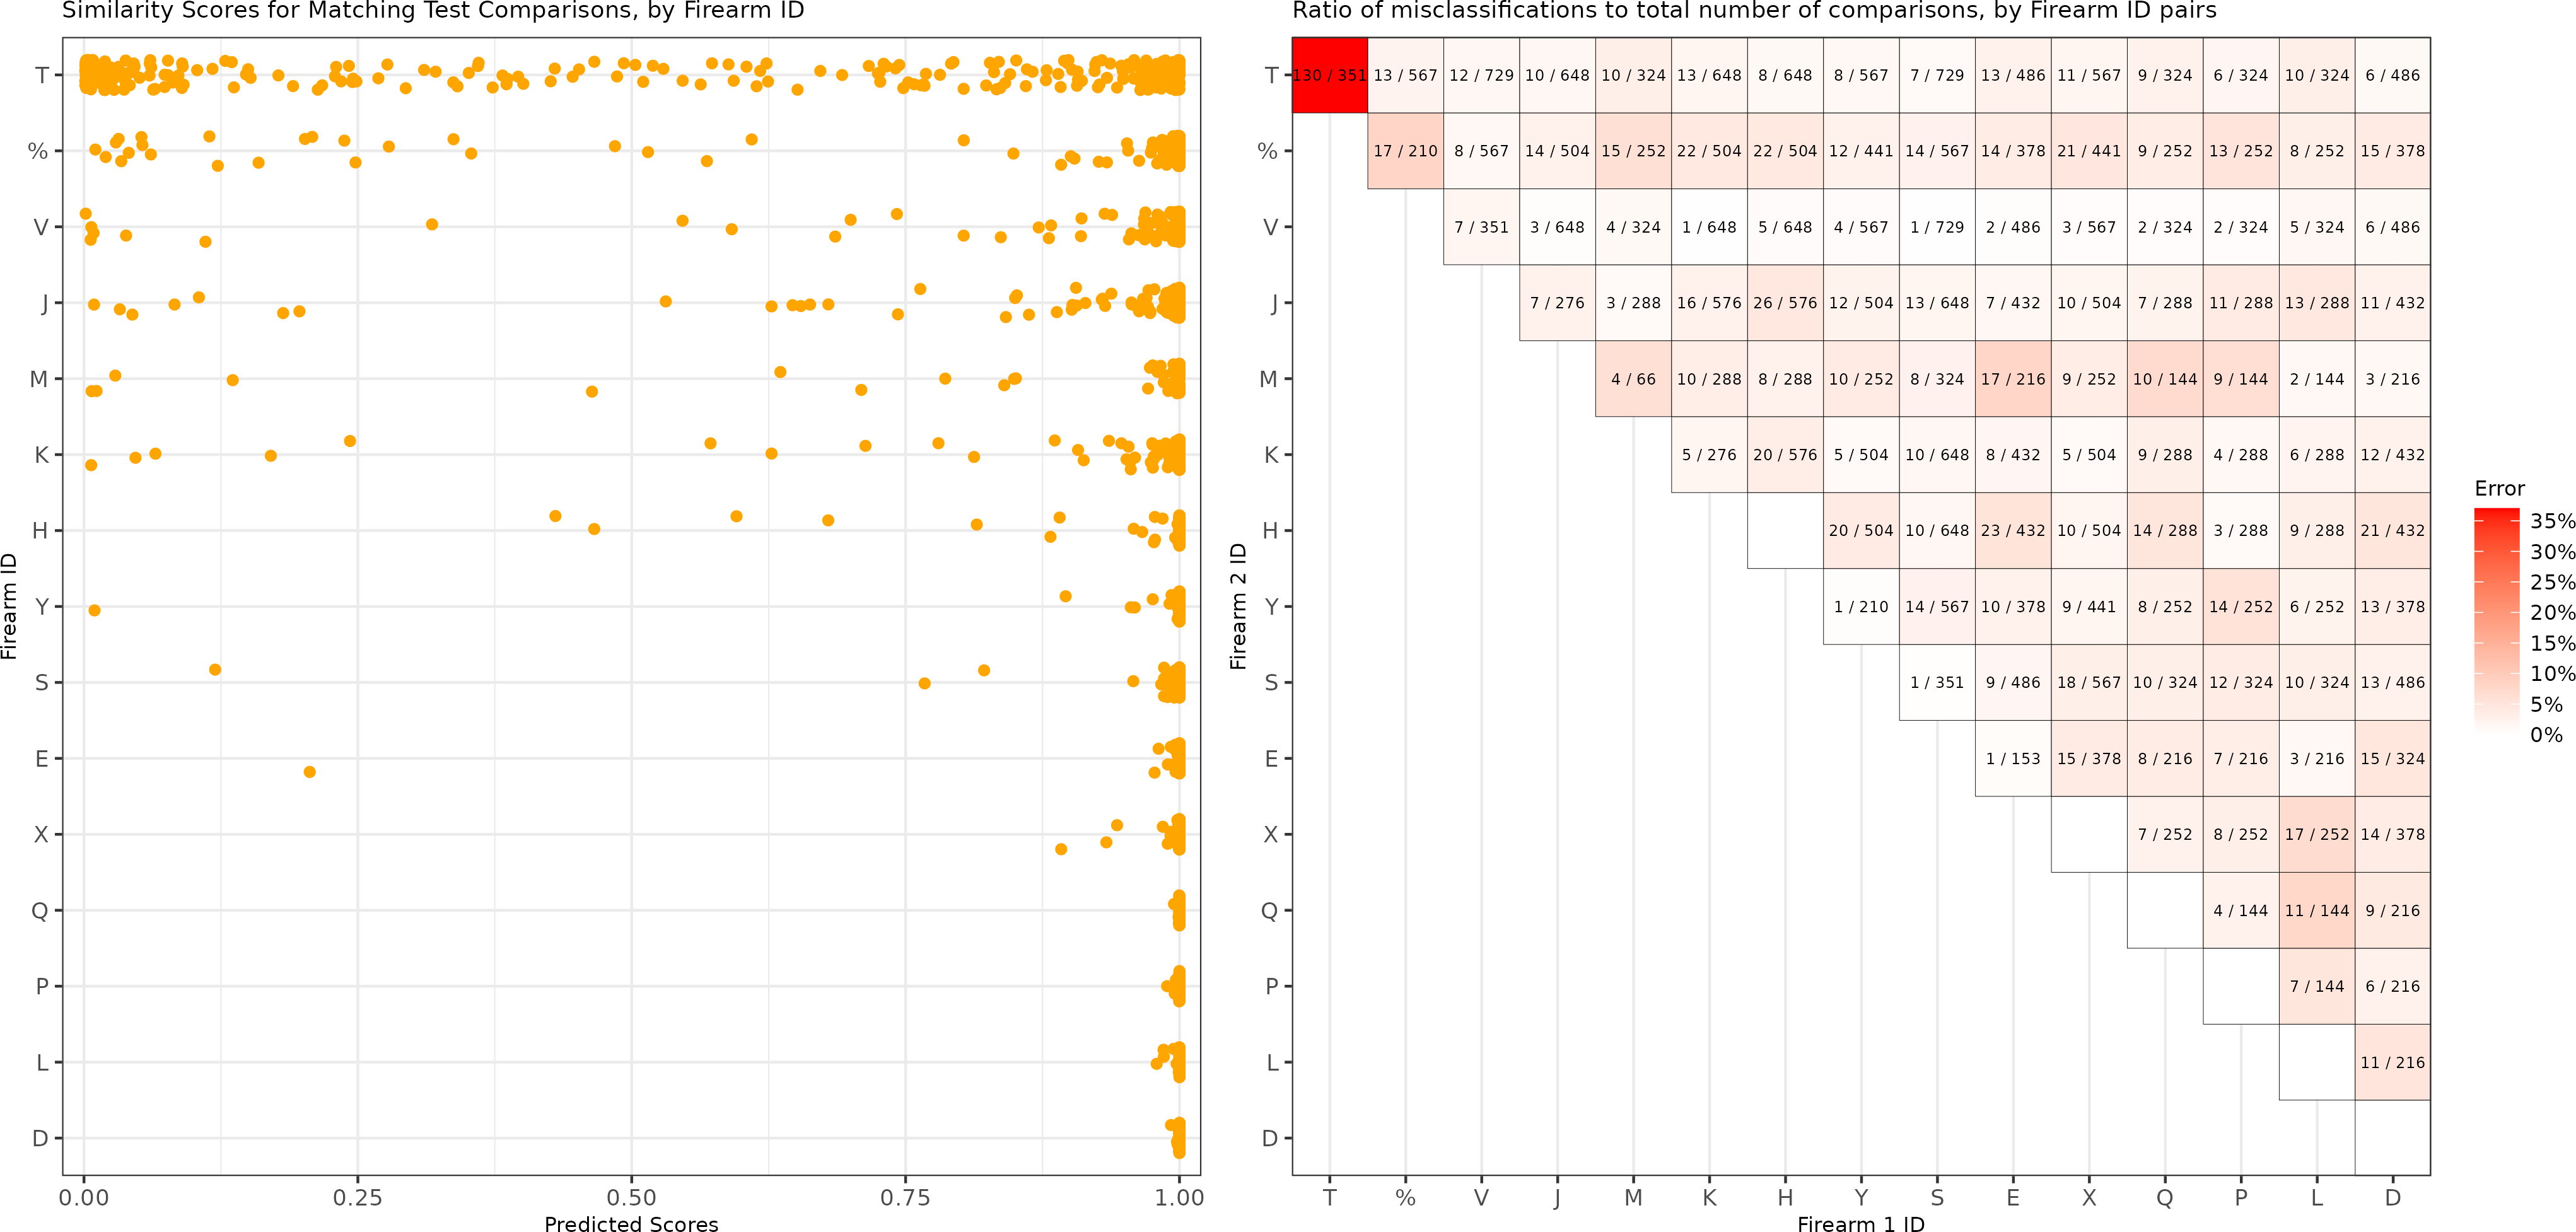
\includegraphics[width=\textwidth]{images/resultsPlots/misclassifPlt} 

}

\caption{\label{fig:testProbs-byFirearm} (Left) A dot plot of the predicted similarity scores for the match comparisons in the test set based on a logistic regression model, separated by firearm. We see that firearm T has more matching comparisons with low similarity scores than the other test firearms. (Right) Misclassifications divided by total number of pairwise comparisons for each pair of test firearms based on the same logistic regression model. We do not show comparisons with 0 misclassifications. We note that the proportion of misclassified matching comparisons from firearm T of 27.1\% is much higher than that of other comparisons.}\label{fig:unnamed-chunk-11}
\end{figure*}

\hypertarget{feature-importance}{%
\subsection{Feature Importance}\label{feature-importance}}

Finally, we consider the relative importance of the 9 features
summarized in \autoref{tab:allFeatures} by fitting 10 replicate random
forests using the full ACES feature set with fixed random seeds. For
each replicate, we measure a variable's importance using the Gini Index,
which measures the probability of making a misclassification for a given
model \citep{hastie_elements_2008}. A larger decrease in the Gini Index
corresponds with higher importance. \autoref{fig:rfVarImpPlt} shows the
distribution of the mean Gini Index decrease for the 9 features. Noting
the log scale on which these points are plotted, we see that the most
important features consist of a combination of density-based features
\(C\) and registration-based correlation features
\(\overline{\text{cor}}_{\text{cell}}\) and
\(\text{cor}_{\text{full}}\). We discuss the sensitivity of these
importance scores to various algorithm parameter choices in the
Appendix.

\begin{figure}[htbp]
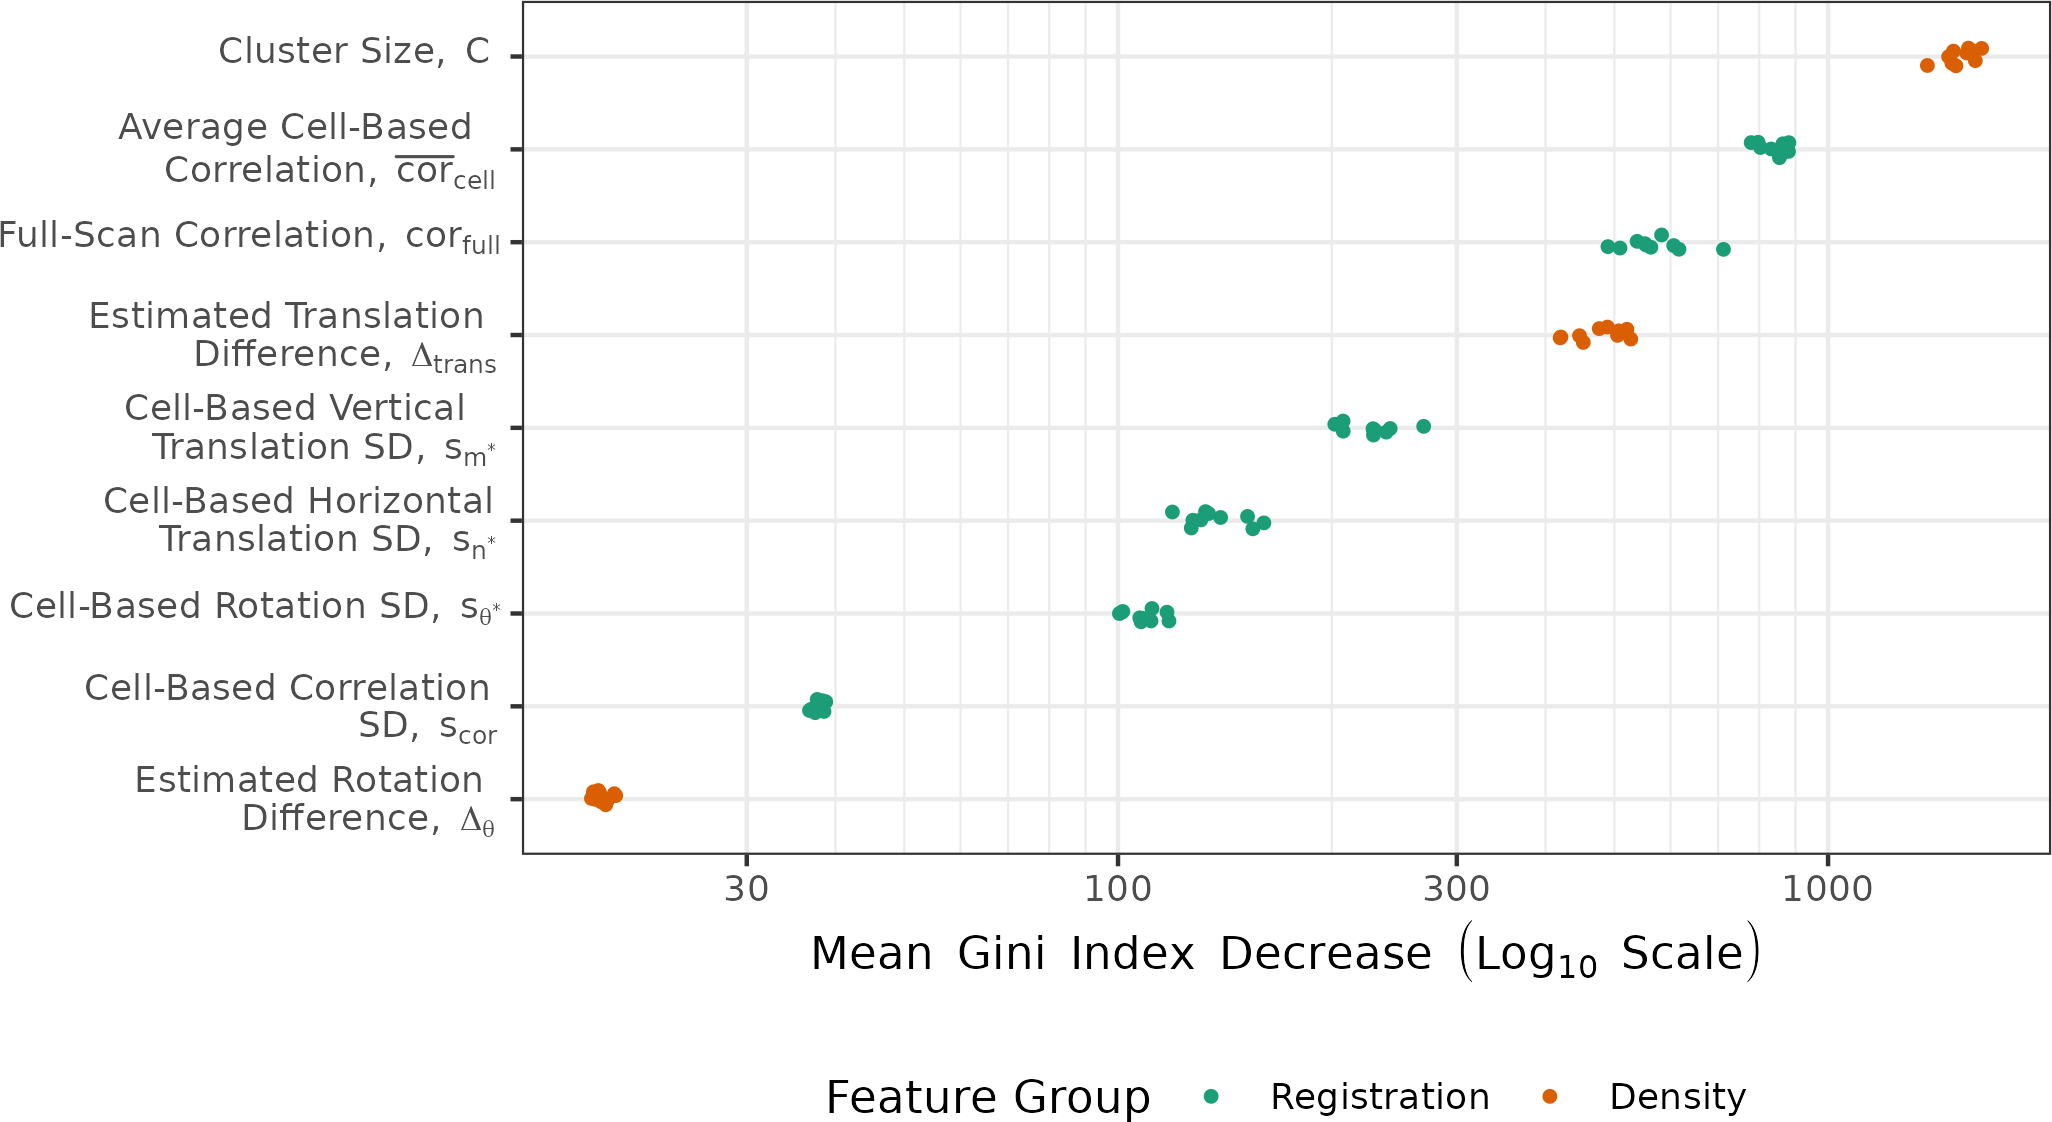
\includegraphics[width=.5\textwidth]{images/resultsPlots/varImpPlt} \caption{\label{fig:rfVarImpPlt} Variable importance measures from fitting a random forest to the training data set, repeated 10 times under various random seeds. The top features consist of  density-based features $C$ and $\Delta_{\text{trans}}$ and registration-based features $\overline{\text{cor}}_{\text{cell}}$ and $\text{cor}_{\text{full}}$. We plot points on a log scale and vertically jitter them for visibility.}\label{fig:unnamed-chunk-12}
\end{figure}

\hypertarget{discussion}{%
\section{Discussion}\label{discussion}}

\hypertarget{comparison-to-cmc-methodology}{%
\subsection{Comparison to CMC
Methodology}\label{comparison-to-cmc-methodology}}

We use Cluster Indicator classifier as a baseline because it is
analogous to the classification rule proposed in
\citet{zhang_convergence_2021}. Similarly, the cell-based registration
features are based on the the same cell-based comparison procedure used
in \citet{song_proposed_2013} and summarized in cell-based comparison.
Together, we consider these classifiers as representing previously
proposed cartridge case similarity scoring algorithms.
\autoref{tab:previousWorkComparison} summarizes the similarities between
our method and the algorithms proposed in \citet{zhang_convergence_2021}
and \citet{song_proposed_2013}. In our view, a defining characteristic
of the previously proposed methods is they make classifications based on
a set of binary decisions; for example, a cell is classified as a
Congruent Matching Cell if its estimated registration is ``close to'' a
reference value where ``closeness'' means being within some pre-defined,
manually chosen threshold of the reference \citep{song_proposed_2013}.
The Cluster Indicator classifier used in \citet{zhang_convergence_2021}
uses the DBSCAN algorithm to compare cell registrations \emph{to each
other} rather than to a reference, but makes classifications based on
the simple rule of whether a cluster is identified among the cell
registrations. In contrast, our approach uses similar information to
these previously proposed, ``rule-based'' methods, but in a more nuanced
manner. We compute continuous summary statistics of the cell
registrations rather than comparing them to a reference value as in the
CMC method. We use the size of the DBSCAN clusters as a feature rather
than simply considering whether a cluster exists as in the Cluster
Indicator classifier. Our approach also combines the cell registration
summaries and DBSCAN cluster features across both comparison directions,
which protects against the rare, but not impossible, chance of a
non-match pair that happens to appear similar in one, but not both,
comparison directions. Finally, the procedure by which we fit a
statistical classifier model using a training feature set has a number
of benefits: (1) model parameters are automatically determined based on
optimizing a set of criteria, (2) it's easier to understand the
relationship between input features and the output score/classification
by considering variable importance or weights, and (3) the continuous,
model-based similarity score provides additional nuance than a discrete
or binary similarity score.

\begin{table*}[htbp]
\centering
\begin{tabular}{p{.18\linewidth} p{.23\linewidth} p{.23\linewidth} p{.23\linewidth}}
Original Paper & Similarities to ACES & Original Use & ACES Use \\
\hline
\citet{song_proposed_2013} & Use \autoref{alg:cellComparison} to estimate cell-based registrations & Call cells Congruent Matching Cells if their registrations are close to a reference value. Classify a cartridge case pair as a match if the CMC count is at least 6. & Compute six summative features based on full-scan and cell registrations. Use features in a classifier model. \\
\hline
\citet{zhang_convergence_2021} & Use DBSCAN algorithm to identify cells that reach a consensus registration & Classify a cartridge case pair as a match if a DBSCAN cluster is identified. & Compute four numerical features based on DBSCAN clusters across both comparison directions. Use features in a classifier model.
\end{tabular}
\caption{Comparison of our approach to previous work. Although our approach shares similarities to previously-proposed algorithms, it includes additional nuance by computing features across both comparison directions and using these features in model-based classifier.}
\label{tab:previousWorkComparison}
\end{table*}

\textbf{Comparison to decision tree model}

\hypertarget{model-selection-considerations}{%
\subsection{Model Selection
Considerations}\label{model-selection-considerations}}

Our intention in fitting the logistic regression and random forest
classification models is to explore each model's strengths and
weaknesses. A critical step in putting cartridge case comparison
algorithms into practice will be to settle on a single model.
Pragmatically, it seems reasonable to choose the model with the highest
estimated accuracy on available test data. However, we noted that models
trained by this optimization criterion on imbalanced data tend to
over-classify the majority class. This is the case for all four
classifiers summarized in \autoref{fig:trainTestAccuracy} despite our
efforts to use supsampling and optimization approaches to mitigate this
effect. If we were instead shift the similarity score classification
threshold for the logistic regression model to maximize the overall
accuracy on the training data, the resulting score threshold is 0.903
with test accuracy, true negative, and true positive rates of 99.2\%,
99.8\%, and 90.0\%, respectively. Given the large true negative rate, we
might favor this model from an ethical perspective since misclassifying
a truly non-matching cartridge case pair may incriminate an innocent
individual. However, the true positive rate is considerably lower than
the ``balanced'' results summarized in \autoref{fig:trainTestAccuracy}.
Further exploration of different optimization criteria is warranted.

Another aspect to consider when choosing a model is interpretability and
explainability. If an algorithm is applied in forensic casework, then
evidentiary conclusions derived from the algorithm's output will
inevitably be presented to a non-expert judge or jury. More
interpretable models are easier to understand, and therefore should be
preferred. The classification behavior of the logistic regression and
classification tree models are arguably easier to explain than the
random forest model. For example, the logistic regression model
parameters can be understood in terms of the estimated increase in odds
of a match. Paired with its comparable performance to the random forest,
we propose the logistic regression model as the preferred model that
balances interpretability with accuracy.

\hypertarget{conclusion}{%
\section{Conclusion}\label{conclusion}}

In this paper, we introduced a novel algorithm to measure the similarity
between two fired cartridge cases based on their breech face
impressions. In particular, we defined a set of 9 similarity features
and used these features to train and test classifier models. We
validated our algorithm on a set of 510 cartridge cases. Compared to
predominant algorithms like the CMC algorithm described in
\citet{song_proposed_2013}, the ACES logistic regression model achieves
higher test accuracy rates while having more balanced true positive and
true negative rates. We propose a logistic regression classifier trained
on the ACES feature set as a new benchmark to which future scoring
methods are compared.

Before our method can be put into practice, we must devise new
stress-tests, using new ammunition and firearm combinations, to assess
its robustness. There is also an opportunity to optimize additional
parameters, such as the number of cells used in cell-based comparison or
parameters used in pre-processing, to measure their effects on final
results. A variety of factors, such as make/model and wear of the
evidence or the algorithm parameters used, affect the discriminative
power of the 19 features defined in this paper. We view the current
version of the ACES algorithm as more a foundation for future
improvements than a final solution. We expect the feature set to evolve
over time; for discriminatory features to supplant less informative
features. Given the gravity of the application, we stress
interpretability as a guiding principle for future feature engineering
and model selection. A misunderstood feature or result may lead a lay
judge or juror to an incorrect conclusion. Additionally, we urge future
researchers to use a train/test procedure similar to the one outlined in
this paper to validate proposed methods.

We developed the \href{https://jzemmels.github.io/scored/}{scored} R
package as an open-source software companion to this paper. The code and
data used in this paper are available at
\url{https://github.com/jzemmels/rules_vs_scores}.

\begin{acknowledgments}
This work was partially funded by the Center for Statistics and
Applications in Forensic Evidence (CSAFE) through Cooperative Agreement
70NANB20H019 between NIST and Iowa State University, which includes
activities carried out at Carnegie Mellon University, Duke University,
University of California Irvine, University of Virginia, West Virginia
University, University of Pennsylvania, Swarthmore College and
University of Nebraska, Lincoln.

We would like to thank the technicians and staff at the Roy J. Carver
High Resolution Microscopy Facility for collecting the topographical
scans used in this paper.

\end{acknowledgments}

\begin{appendices}

\section{Training Feature Distributions}

\begin{figure}[htbp]
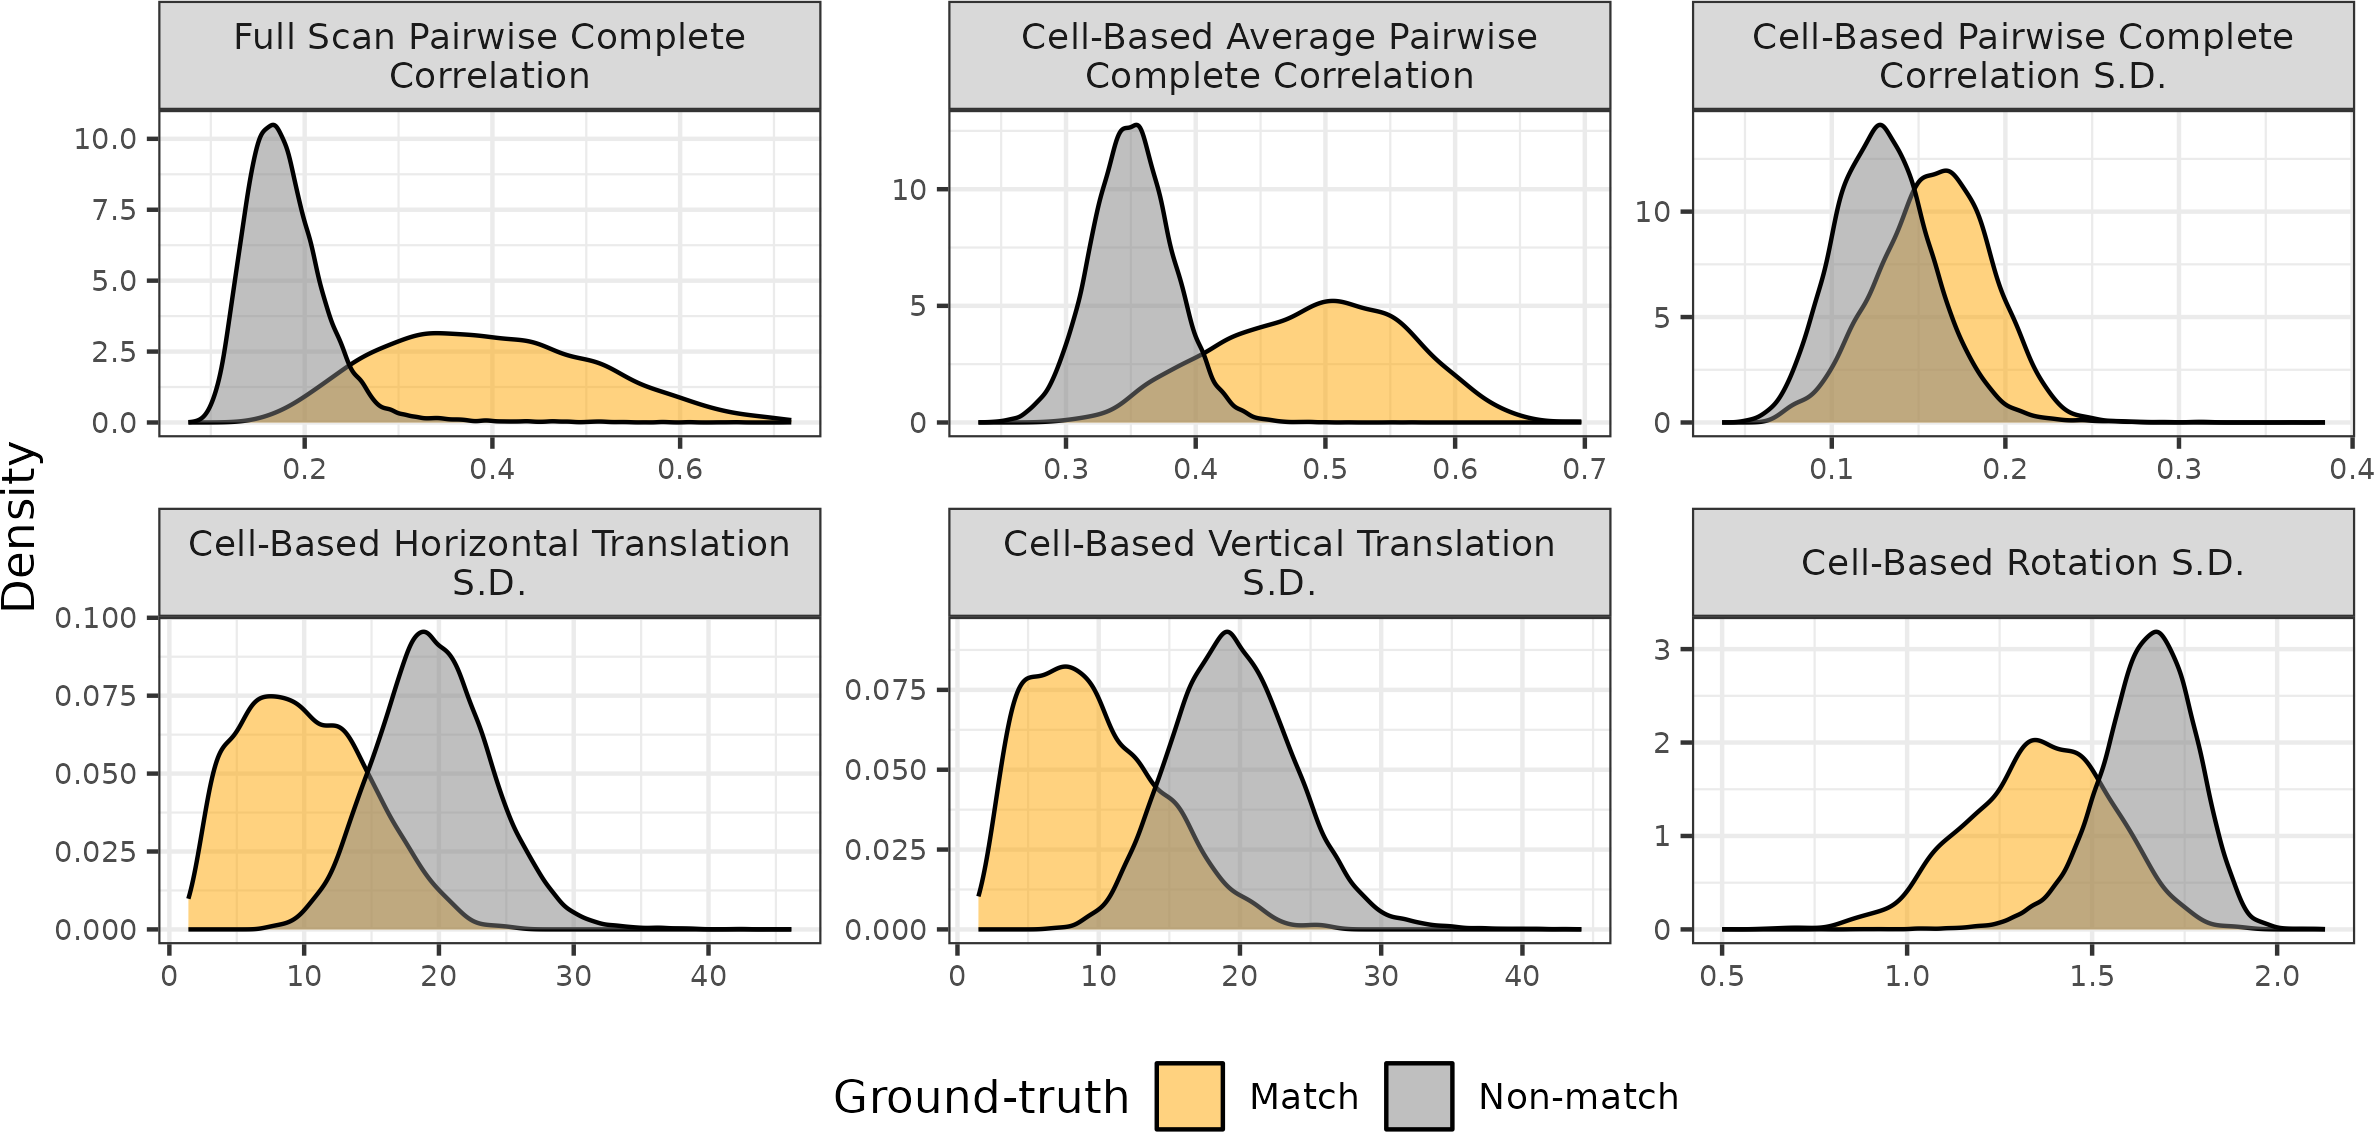
\includegraphics[width=.5\textwidth]{images/resultsPlots/featureDensity_registration} \caption{Density plots of the Registration-Based features for 21,945 cartridge case pairs. The standard deviation of the cell-based registrations distinguish between match and non-match pairs better than the mean values.}\label{fig:registrationDensities}
\end{figure}

\begin{figure}[htbp]
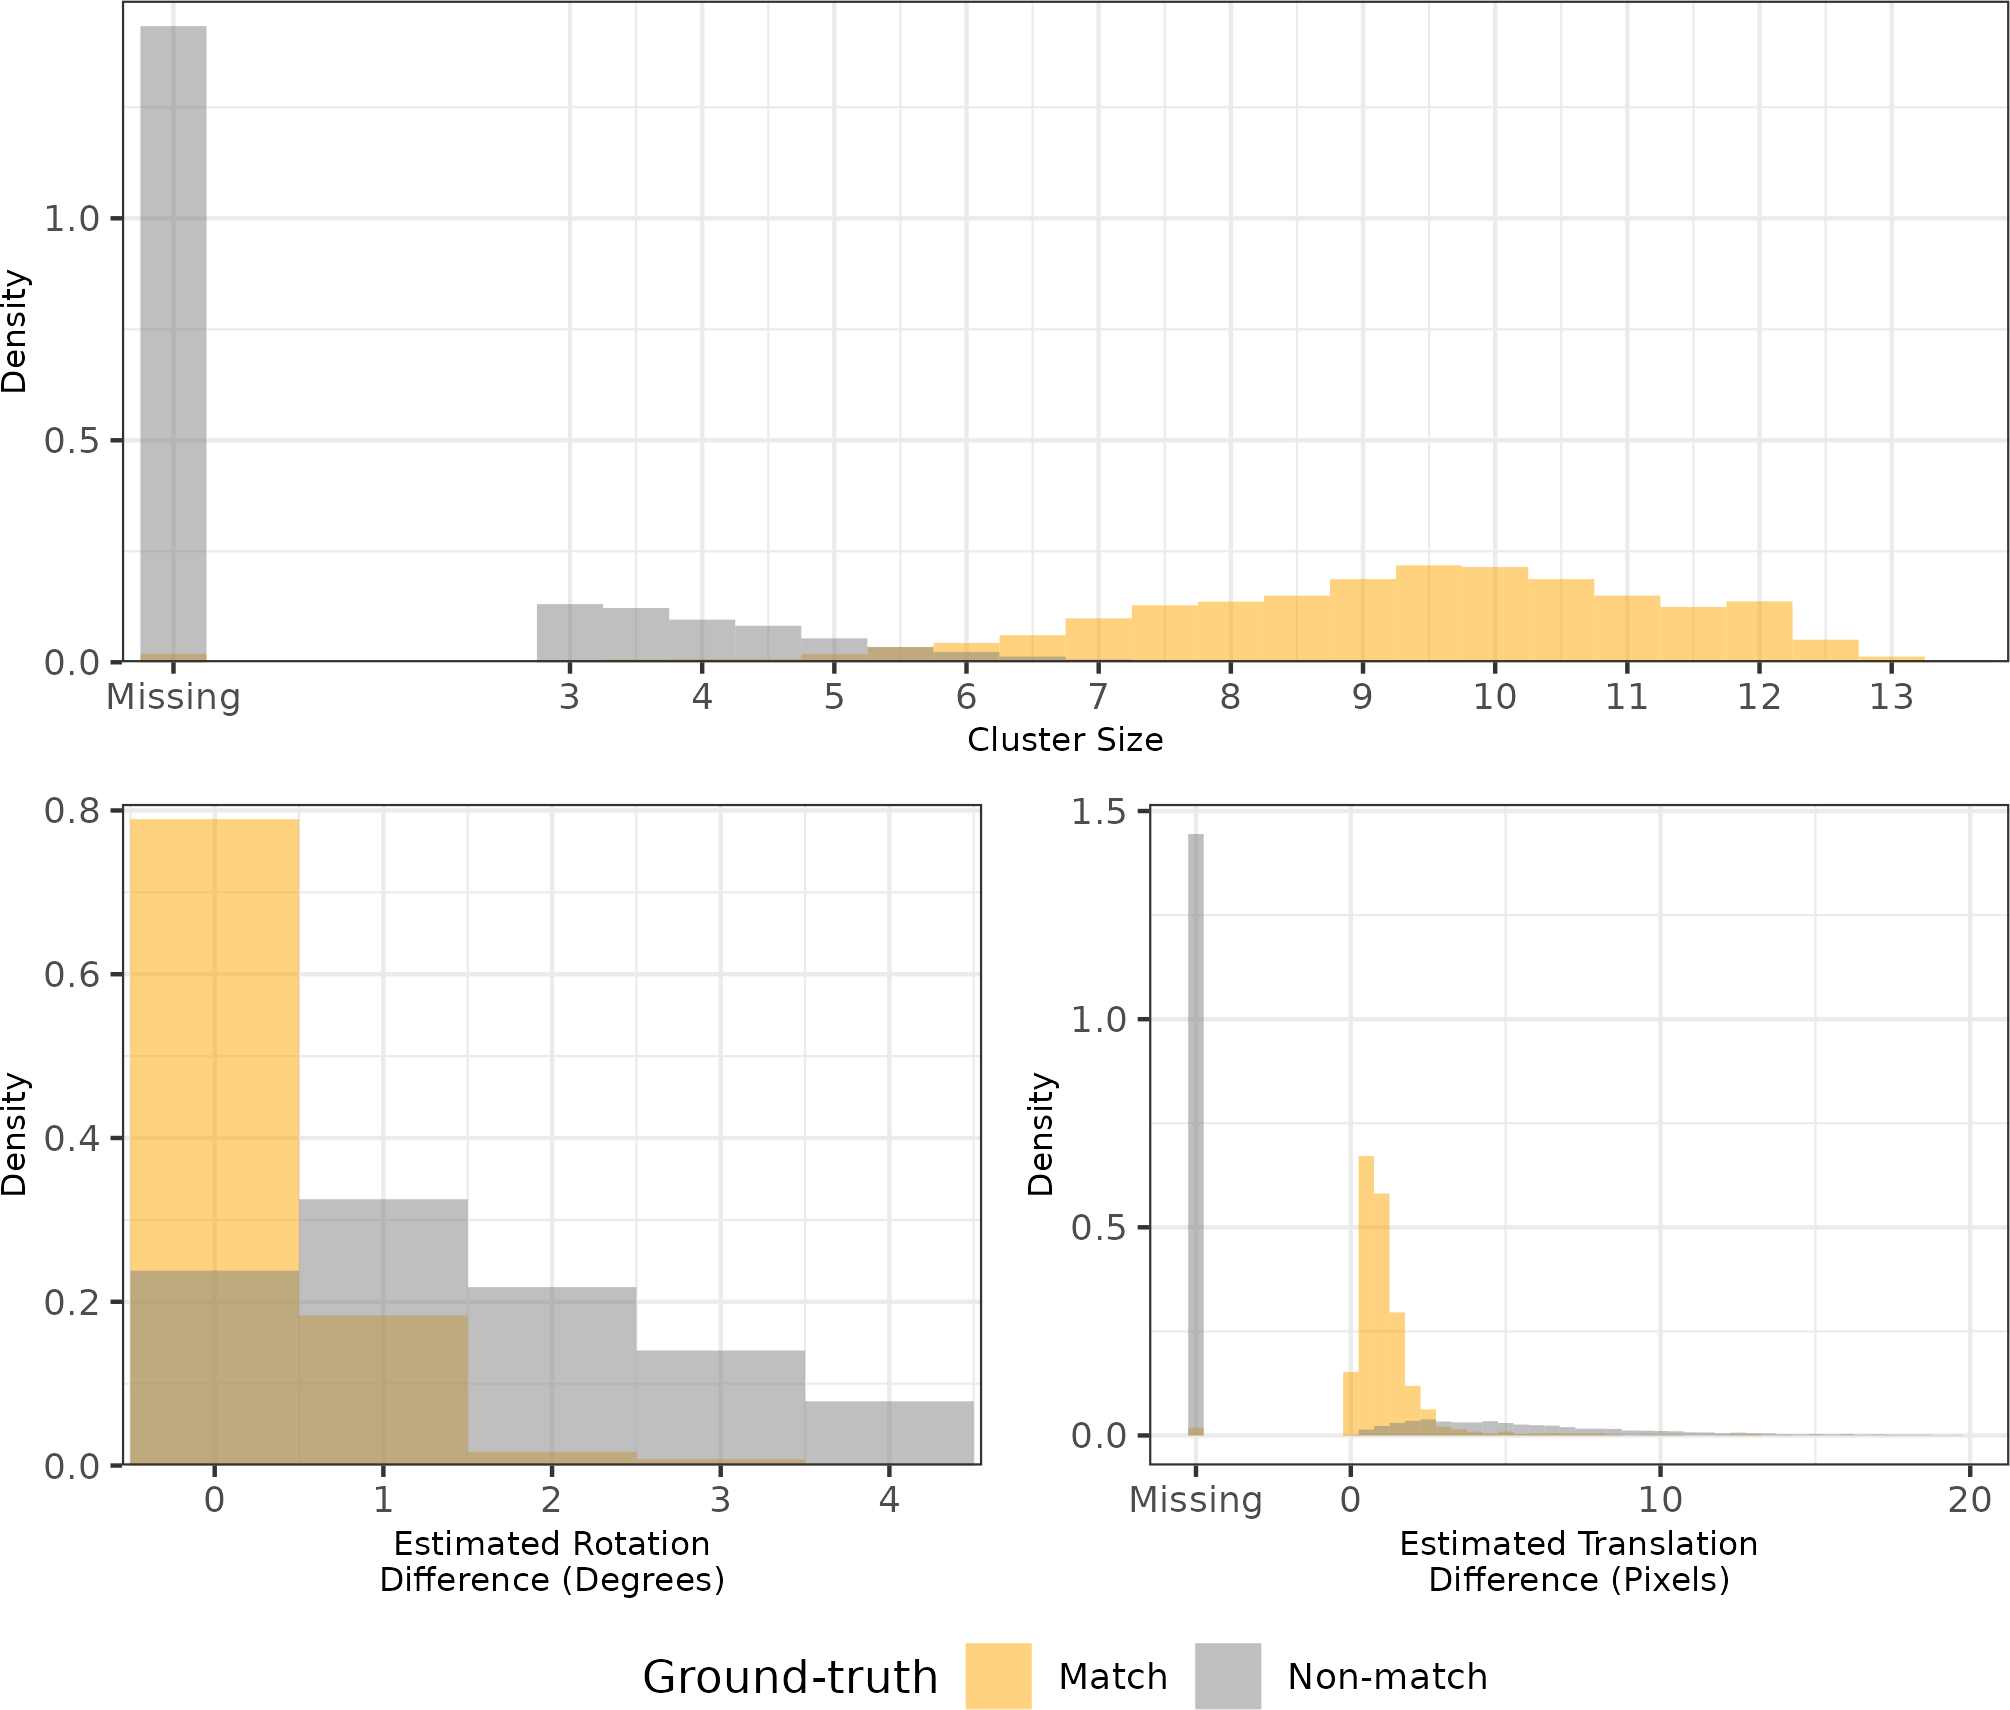
\includegraphics[width=.5\textwidth]{images/resultsPlots/featureDensity_densityBased} \caption{Distributions of the density-based features for 21,945 cartridge case pairs. The Cluster Size and Estimated Translation Difference features may be missing (\texttt{NA}) if no DBSCAN cluster is identified, which commonly occurs for non-matching cartridge case pairs as evidenced by the stacked bar chart in the top left.}\label{fig:densityDistributions}
\end{figure}

\section{Model Results}

\begin{table}[htbp]
    \centering
    \begin{tabular}{l|r|r|r}
         \textbf{Classifier} & \textbf{Accuracy} & \textbf{True Negative} & \textbf{True Positive} \\
         \hline
         Cluster Ind. & 90.5\% & 90.4\% & 90.7\% \\
         CMC & 88.6\% & 89.0\% & 86.9\% \\
         \hline
         LR & 97.5\% & 97.5\% & 97.5\% \\
         RF & \textbf{99.6\%} & \textbf{99.6\%} & \textbf{99.6\%}
    \end{tabular}
    \caption{Training accuracy, true positive, and true negative rates for the 4 binary classifiers. This table shows a numeric summary of the results shown in the Results section. We bold the largest values in each column for emphasis.}
    \label{tab:trainDataResults}
\end{table}

\begin{table}[htbp]
    \centering
    \begin{tabular}{l|r|r|r}
         \textbf{Classifier} & \textbf{Accuracy} & \textbf{True Negative} & \textbf{True Positive} \\
         \hline
         Cluster Ind. & 89.4\% & 89.6\% & 86.8\% \\
         CMC & 96.9\% & 98.8\% & 71.0\% \\
         \hline
         LR & 97.3\% & 97.5\% & \textbf{94.4\%} \\
         RF & \textbf{98.9\%} & \textbf{99.3\%} & 92.2\%
    \end{tabular}
    \caption{Test accuracy, true positive, and true negative rates for the 4 binary classifiers. This table shows a numeric summary of the results shown in the Results section. We bold the largest values in each column for emphasis.}
    \label{tab:testDataResults}
\end{table}

\section{Congruent Matching Cells Algorithm Criteria} \label{appendixCMC}

This section will provide a more thorough definition of the classification criteria used in the Congruent Matching Cells algorithm as proposed in \citet{song_proposed_2013}.
This section assumes that the reader is familiar with the notation and algorithms, \autoref{alg:registration} and \autoref{alg:cellComparison}, introduced in \ref{methods}.

\end{appendices}

% -------------------------------------------------------------------------------------------------------------------
%   Appendix  (optional)

%\appendix
%\section{Appendix title}

%If only one appendix, please use
%\appendix*
%\section{Appendix title}


%=======================================================

%Use \bibliography{<name of your .bib file>}+
%to make your bibliography with BibTeX.

%=======================================================

\bibliography{biblio.bib}


\end{document}
